\documentclass[11pt,letterpaper,oneside]{report}

% ---------------------------------------------------------------- Paquetes
\usepackage[utf8]{inputenc}
\usepackage[T1]{fontenc}
\usepackage[spanish,es-tabla,es-nodecimaldot]{babel}
\usepackage{lmodern}
\usepackage[margin=2.5cm]{geometry}
\usepackage{amsmath}
\usepackage{graphicx}
\usepackage{subcaption}
\usepackage{booktabs}
\usepackage{array}
\usepackage{longtable}
\usepackage{float}
\usepackage[section]{placeins}
\usepackage{enumitem}
\usepackage{listings}
\usepackage[hyphens]{url}
\usepackage{parskip}          % párrafos sin sangría
\usepackage{xcolor}
\usepackage{rotating}
\usepackage{titlesec}
\usepackage[hidelinks]{hyperref}   % enlaces activos, todo el texto en negro

% Títulos de capítulo sin la palabra "Capítulo": solo número y nombre
\titleformat{\chapter}[hang]{\normalfont\huge\bfseries}{\thechapter.}{0.6em}{}
\titlespacing*{\chapter}{0pt}{0pt}{18pt}

% Nombres en español (por si el idioma de babel no los define)
\AtBeginDocument{%
  \renewcommand{\contentsname}{Índice}%
  \renewcommand{\bibname}{Referencias}%
  \renewcommand{\figurename}{Figura}%
  \renewcommand{\tablename}{Tabla}%
  \renewcommand{\appendixname}{Anexo}%
  \renewcommand{\lstlistingname}{Código}%
}

\graphicspath{{img/}}
\newcommand{\um}{\ensuremath{\mu}m}
\newcommand{\code}[1]{\texttt{#1}}
\newcommand{\repo}{https://github.com/SebastianRodriguez05/risc-v-manizales/tree/main}

\lstset{basicstyle=\ttfamily\small\color{black}, columns=fullflexible, keepspaces=true,
        breaklines=true, tabsize=4, showstringspaces=false,
        frame=single, rulecolor=\color{black!25}, backgroundcolor=\color{black!3},
        xleftmargin=4pt, xrightmargin=4pt, aboveskip=6pt, belowskip=6pt,
        literate={á}{{\'a}}1 {é}{{\'e}}1 {í}{{\'i}}1 {ó}{{\'o}}1 {ú}{{\'u}}1 {ñ}{{\~n}}1}

\setlist{itemsep=2pt, topsep=4pt}
\emergencystretch=2.5em

\title{\textbf{Pruebas del procesador femto\_UN}\\[6pt]
\Large Diseño fabricado en Tiny Tapeout, arranque con memoria flash emulada\\ y prueba de la memoria RAM SPI}
\author{Femto-UN\\ Universidad Nacional}
\date{Noviembre de 2026}

\begin{document}
\maketitle
\tableofcontents

% ======================================================================
\chapter{Introducción}

\section{Contexto}

El femto\_UN es un procesador RISC-V de 32 bits basado en el núcleo femtoRV32 Quark (RV32I) de Bruno Levy, fabricado como circuito integrado a través del programa Tiny Tapeout con el nombre de proyecto \code{tt\_um\_femto}. El chip llega montado en la placa de demostración de Tiny Tapeout, que incluye un microcontrolador RP2040 encargado de seleccionar el proyecto, generar el reloj y controlar el reset, y que expone las entradas y salidas del chip en conectores PMOD.

El femto\_UN no tiene memoria interna: lee su programa desde una memoria flash externa por un bus SPI, usa una memoria RAM externa por un segundo bus SPI y se comunica con el exterior por una UART. Para verlo funcionar hay que resolver tres cosas fuera del chip: de dónde lee el programa, cómo se conecta todo lo que lo rodea y cómo se comprueba que lo que hace coincide con lo que se diseñó.

Este documento reúne las pruebas realizadas al procesador: primero presenta el diseño que se envió a fabricar, luego el montaje físico, el primer arranque con una memoria flash emulada y, por último, la prueba de la memoria RAM.

\section{Objetivo}

Poner en marcha el procesador femto\_UN en hardware real y dejar documentado el camino seguido, de modo que cada prueba pueda entenderse y repetirse. En concreto, el trabajo buscó:

\begin{itemize}
  \item Documentar el diseño fabricado a partir de su layout final: vistas 2D y 3D y resultados de implementación.
  \item Lograr que el femto\_UN arranque desde una memoria de programa y envíe un mensaje por la UART, usando un ESP32-C6 como memoria flash SPI emulada.
  \item Comprobar el bus de la memoria RAM del chip, leyendo, escribiendo y conservando datos en una memoria F-RAM FM25V02.
\end{itemize}

\section{Resultados principales}

\begin{itemize}
  \item El layout fabricado ocupa 4$\times$2 tiles (682,64 $\times$ 225,76\,\um) en SkyWater 130\,nm, dentro del shuttle TTSKY25b, y pasó todas las verificaciones previas al envío.
  \item El femto\_UN arrancó en hardware y envió \code{Hello World from femto UN} por la UART, con el ESP32-C6 como memoria de programa y un reloj de 100\,kHz.
  \item El femto\_UN leyó, escribió y conservó datos en la RAM, y ejecutó un programa que guarda texto en ella y lo devuelve en mayúsculas. Como el controlador del chip no envía el comando de habilitación de escritura, ese comando se genera desde el programa.
  \item En ese proceso se identificó cómo se comporta el bus SPI del chip fabricado y qué condiciones debe cumplir la memoria para que el procesador arranque: responder solo al comando de lectura y dejar la línea MISO en alto cuando está en reposo.
\end{itemize}

\section{Herramientas y equipos}

La Tabla~\ref{tab:herramientas} resume lo usado a lo largo de las pruebas. Todo el desarrollo se hizo en Fedora Linux.

\begin{table}[htbp]
\centering
\caption{Herramientas y equipos usados.}
\label{tab:herramientas}
\begin{tabular}{>{\raggedright\arraybackslash}p{6.2cm} >{\raggedright\arraybackslash}p{8.4cm}}
\toprule
\textbf{Herramienta o equipo} & \textbf{Uso} \\
\midrule
Placa de demostración de Tiny Tapeout & Soporte del chip femto\_UN, reloj y reset \\
ESP32-C6-WROOM-1 & Memoria flash SPI emulada \\
FM25V02 (F-RAM de 32\,KB) & Memoria RAM SPI \\
Adaptador USB-UART FTDI & Lectura de la UART del chip \\
Analizador lógico y PulseView & Captura de las señales SPI y UART \\
\code{riscv-none-elf-gcc} & Compilación del firmware del procesador \\
\code{arduino-cli} & Carga del emulador en el ESP32-C6 \\
\code{mpremote} y \code{minicom} & Consola de la placa de demostración y terminal de la UART \\
Visor 3D de Tiny Tapeout y KLayout & Vistas del layout fabricado \\
\bottomrule
\end{tabular}
\end{table}

\section{Organización del documento}

El Capítulo~\ref{cap:fabricado} presenta el diseño enviado a fabricación: su layout en 2D y 3D y los resultados de implementación. El Capítulo~\ref{cap:montaje} describe el montaje físico con el que se hicieron todas las pruebas. El Capítulo~\ref{cap:flash} explica el uso del ESP32-C6 como memoria flash del femto\_UN y la prueba con la que el chip arrancó y envió su primer mensaje, incluido el análisis del bus SPI del chip. El Capítulo~\ref{cap:ram} presenta la prueba de la memoria RAM: cómo se resolvió desde el programa la falta del comando de habilitación de escritura, la prueba de lectura, escritura y persistencia, y el programa que convierte texto a mayúsculas. El Capítulo~\ref{cap:conclusiones} recoge las conclusiones y los cambios propuestos para una segunda versión del procesador.

\section{Repositorios}

El material de las pruebas está en el repositorio \href{https://github.com/SebastianRodriguez05/risc-v-manizales}{risc-v-manizales}, donde cada prueba tiene su propia carpeta con un archivo \code{README.md}. El diseño fabricado y su copia de referencia están en el repositorio de la organización, \href{https://github.com/Femto-UN/riscv-vlsi}{Femto-UN/riscv-vlsi}. La Tabla~\ref{tab:repos} indica dónde está el material de cada capítulo.

\begin{table}[htbp]
\centering
\caption{Ubicación del material de cada capítulo.}
\label{tab:repos}
\begin{tabular}{c >{\raggedright\arraybackslash}p{6.4cm} >{\raggedright\arraybackslash}p{6.4cm}}
\toprule
\textbf{Capítulo} & \textbf{Ubicación} & \textbf{Contenido} \\
\midrule
\ref{cap:fabricado} & \href{https://github.com/TinyTapeout/tinytapeout-sky-25b/tree/main/projects/tt_um_femto}{tinytapeout-sky-25b/projects/tt\_um\_femto} & Layout oficial y métricas \\
\ref{cap:fabricado} & \href{https://github.com/Femto-UN/riscv-vlsi}{Femto-UN/riscv-vlsi} & Diseño fabricado y reportes de Tiny Tapeout \\
\ref{cap:flash} & \href{\repo/firmware/esp32_flash_emu}{firmware/esp32\_flash\_emu} & Emulador de flash en el ESP32-C6 \\
\ref{cap:flash} & \href{\repo/asic/hello_world_uart}{asic/hello\_world\_uart} & Primer arranque del femto\_UN \\
\bottomrule
\end{tabular}
\end{table}

% ======================================================================
\chapter{El diseño fabricado}
\label{cap:fabricado}

\section{Descripción}

El diseño ejecuta el programa desde una memoria \textbf{flash SPI} externa, usa una \textbf{RAM SPI} externa como memoria de datos y se comunica por \textbf{UART} para la depuración. Fue desarrollado por el profesor Carlos Iván Camargo Bareño en la Universidad Nacional de Colombia.

El diseño se envió a fabricación en el shuttle \textbf{TTSKY25b} de Tiny Tapeout, sobre el proceso \textbf{SkyWater 130\,nm} (PDK \code{sky130A}). Este shuttle cerró el 10 de noviembre de 2025 con 316 diseños y se envió a la fundición (ChipFoundry) ese mismo mes~\cite{ttsky25b_news}. El flujo físico ---síntesis, colocación, ruteo y verificación--- lo ejecutó de forma automática la GitHub Action de Tiny Tapeout con \textbf{LibreLane 2.4.2}~\cite{gds_run}, a partir del commit \code{baab83f} del repositorio \href{https://github.com/cicamargoba/femto_UN}{cicamargoba/femto\_UN}~\cite{repo_femto}.

Las vistas de este capítulo se tomaron del layout final publicado en el repositorio oficial del shuttle~\cite{repo_shuttle}; las vistas 3D se obtuvieron con el visor 3D de Tiny Tapeout~\cite{tt_chip}. La Tabla~\ref{tab:datos} resume las características del diseño.

\begin{table}[htbp]
\centering
\caption{Datos del diseño fabricado.}
\label{tab:datos}
\begin{tabular}{>{\raggedright\arraybackslash}p{4.6cm} >{\raggedright\arraybackslash}p{9.8cm}}
\toprule
\textbf{Dato} & \textbf{Valor} \\
\midrule
Proyecto & UNAL's RISCV (\code{tt\_um\_femto}) \\
Shuttle & TTSKY25b (Tiny Tapeout) \\
Proceso / PDK & SkyWater 130\,nm, \code{sky130A} (open\_pdks \code{0fe599b}) \\
Librería de celdas & \code{sky130\_fd\_sc\_hd} \\
Flujo & LibreLane 2.4.2 \\
Commit fabricado & \href{https://github.com/cicamargoba/femto_UN/commit/baab83f5b7fe16083744b88fc54fe699873517e1}{\code{baab83f}} (5 de noviembre de 2025) \\
Tamaño & 4$\times$2 tiles: \textbf{682,64 $\times$ 225,76\,\um} (154\,113\,\um$^2$) \\
Restricción de reloj & 25\,ns (40\,MHz) \\
Layout oficial & \href{https://github.com/TinyTapeout/tinytapeout-sky-25b/tree/main/projects/tt_um_femto}{\code{projects/tt\_um\_femto/tt\_um\_femto.oas}} \\
\bottomrule
\end{tabular}
\end{table}

\section{Arquitectura RTL}

La Figura~\ref{fig:rtl} muestra la arquitectura del RTL que se envió a fabricar, tomada del Verilog del commit \code{baab83f}: los seis archivos que lista \code{info.yaml}, idénticos a los que usó el flujo GDS de Tiny Tapeout~\cite{gds_run}. El módulo superior \code{tt\_um\_femto} registra el reset en el flanco de bajada del reloj y contiene el SoC \code{femto}, que une el núcleo FemtoRV32 con tres periféricos mapeados en memoria. Un decodificador usa los 16 bits más altos de la dirección para seleccionar el periférico, y un multiplexor devuelve al núcleo el dato leído.

\begin{figure}[htbp]
\centering
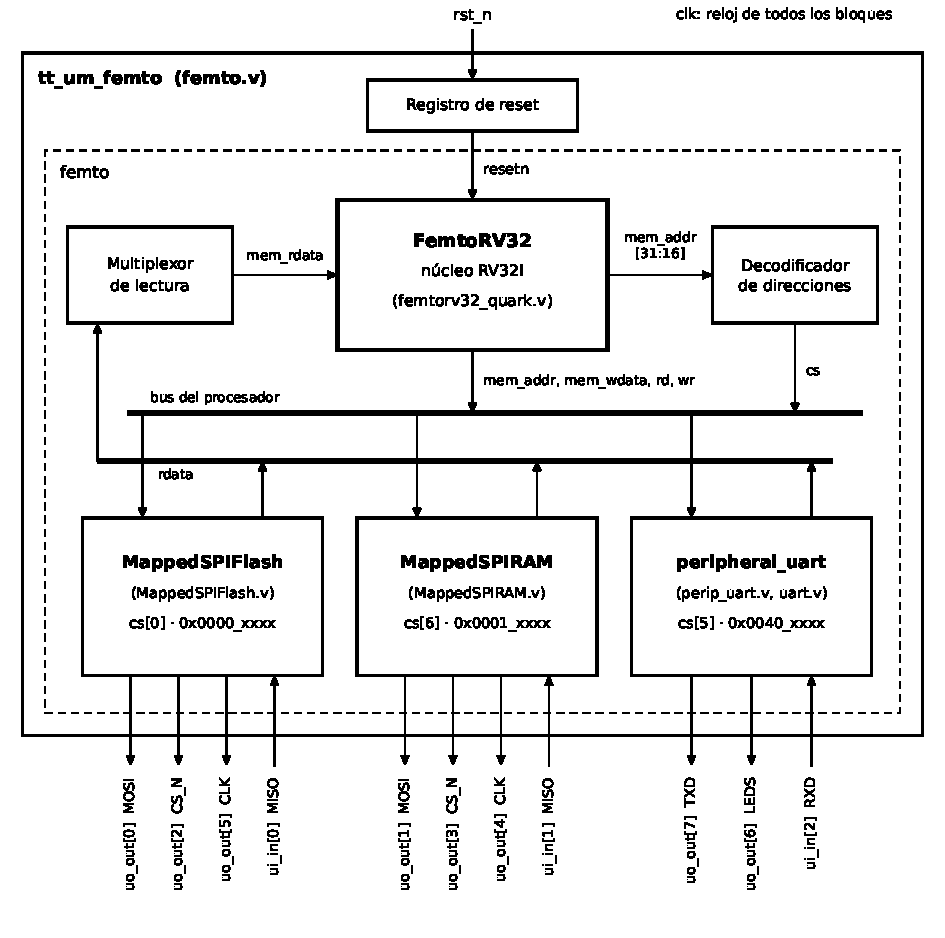
\includegraphics[width=\textwidth]{rtl_femto.pdf}
\caption{Diagrama de bloques del RTL fabricado (\code{femto.v}). Abajo, los pines del chip que usa cada periférico.}
\label{fig:rtl}
\end{figure}

La Tabla~\ref{tab:rtl} resume la función de cada archivo y la región de memoria de cada periférico.

\begin{table}[htbp]
\centering
\caption{Archivos RTL del diseño fabricado.}
\label{tab:rtl}
\begin{tabular}{l r >{\raggedright\arraybackslash}p{8.6cm}}
\toprule
\textbf{Archivo} & \textbf{Líneas} & \textbf{Contenido} \\
\midrule
\code{femto.v} & 190 & Módulo superior \code{tt\_um\_femto} y SoC \code{femto}: decodificador de direcciones, multiplexor de lectura y asignación de pines \\
\code{femtorv32\_quark.v} & 544 & Núcleo RISC-V FemtoRV32 Quark (RV32I) \\
\code{MappedSPIFlash.v} & 137 & Controlador de la flash SPI, direcciones \code{0x0000\_xxxx} \\
\code{MappedSPIRAM.v} & 165 & Controlador de la RAM SPI, direcciones \code{0x0001\_xxxx} \\
\code{perip\_uart.v} & 74 & Periférico de la UART, direcciones \code{0x0040\_xxxx} \\
\code{uart.v} & 162 & Transmisor y receptor UART \\
\bottomrule
\end{tabular}
\end{table}

\section{Vista general del layout}

La Figura~\ref{fig:general2d} muestra el render 2D del layout completo generado por Tiny Tapeout. Los pines del proyecto se conectan por el borde superior con el multiplexor del chip. El recuadro rojo marca, de forma aproximada, la zona que se amplía en la Sección~\ref{sec:zoom}.

\begin{figure}[htbp]
\centering
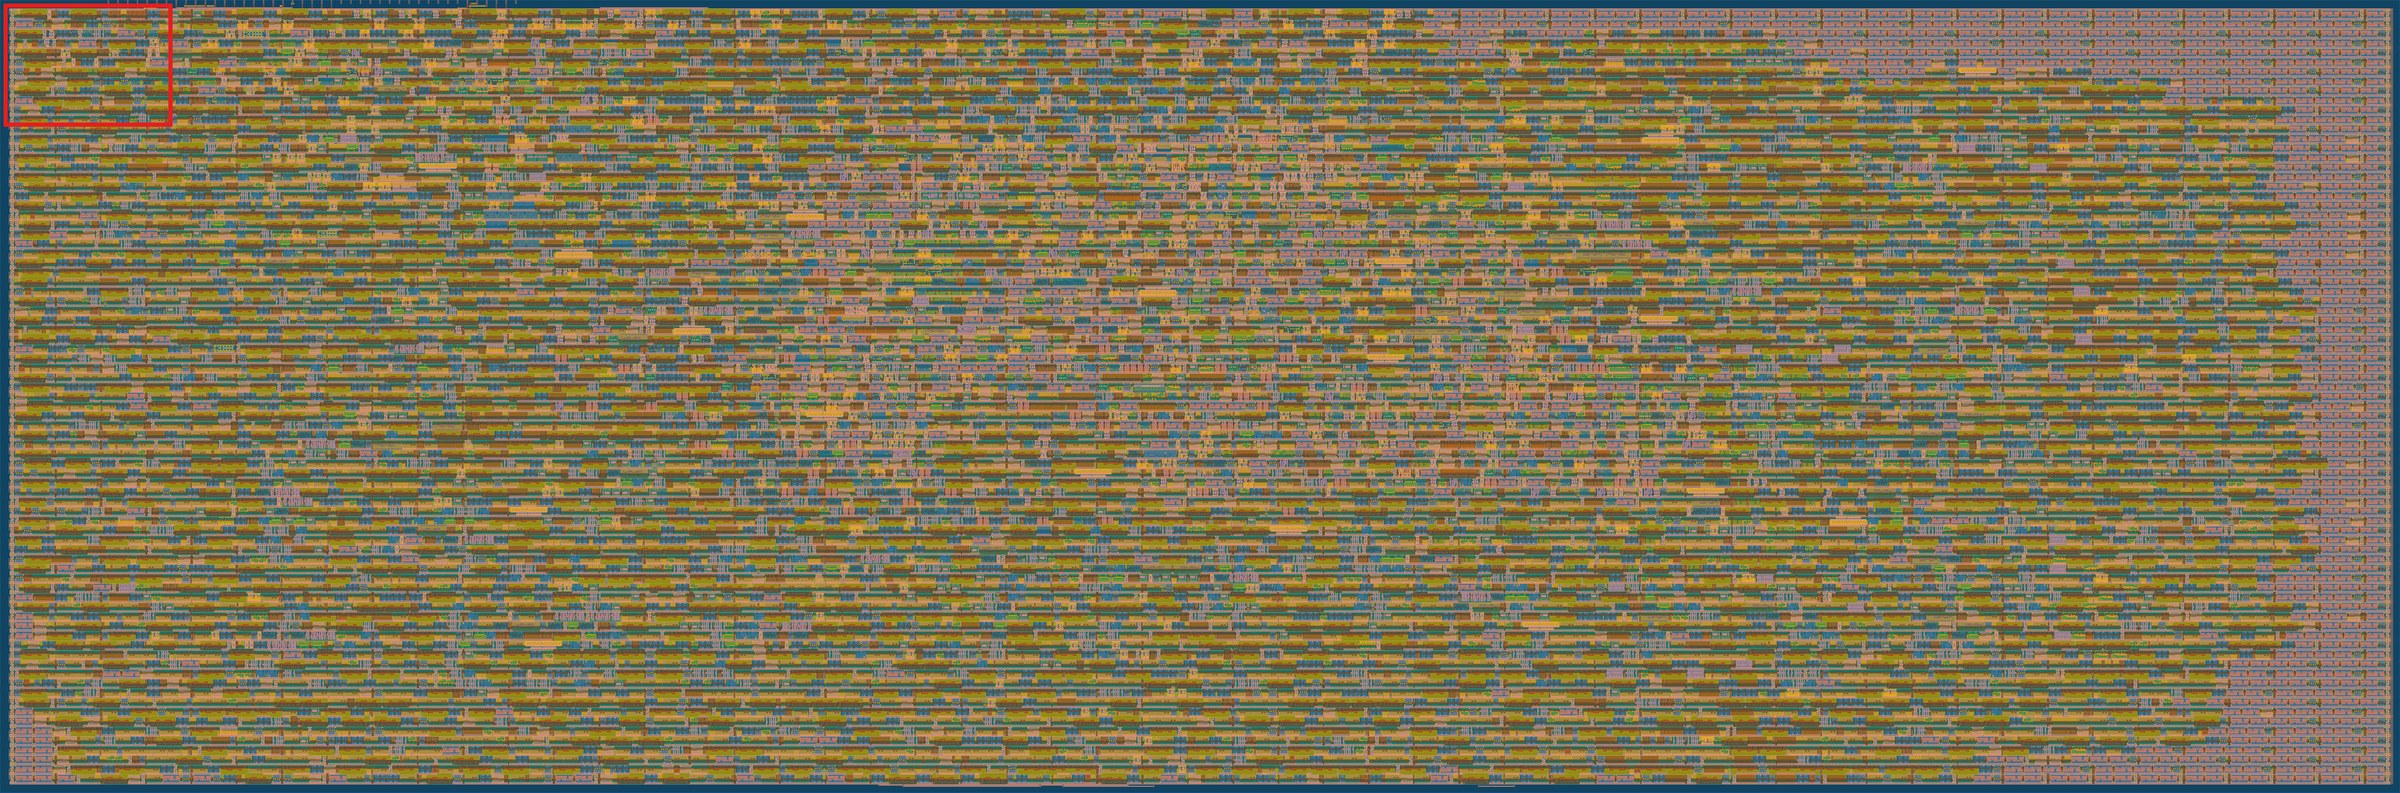
\includegraphics[width=\textwidth]{vista_general_2d_recuadro.jpg}
\caption{Render 2D del layout completo de \code{tt\_um\_femto}. El recuadro rojo indica la zona ampliada en la Figura~\ref{fig:zoom}.}
\label{fig:general2d}
\end{figure}

La Figura~\ref{fig:general3d} presenta el mismo diseño en el visor 3D. Las bandas verticales oscuras corresponden al power grid en metal~4, que distribuye la alimentación a todas las filas de celdas.

\begin{figure}[htbp]
\centering
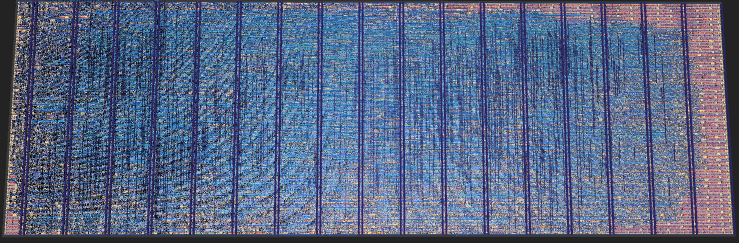
\includegraphics[width=\textwidth]{vista_general_3d.png}
\caption{Vista 3D del layout completo en el visor de Tiny Tapeout.}
\label{fig:general3d}
\end{figure}

\section{Ampliación de la esquina superior izquierda}
\label{sec:zoom}

La Figura~\ref{fig:zoom} muestra una misma zona del diseño con distintas capas visibles. En la librería \code{sky130\_fd\_sc\_hd} cada fila de celdas mide 2,72\,\um{} de alto, por lo que la zona mostrada tiene cerca de 33\,\um{} de alto.

\begin{figure}[htbp]
\centering
\begin{subfigure}[t]{0.48\textwidth}
  \centering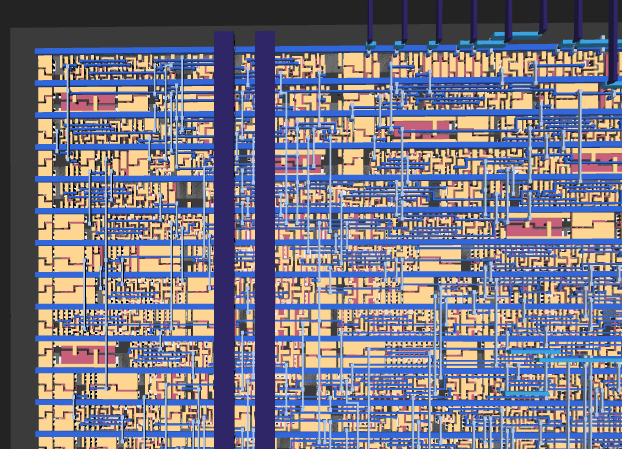
\includegraphics[width=\linewidth]{zoom_3d_completo.png}
  \caption{Todas las capas.}\label{fig:zoom_a}
\end{subfigure}\hfill
\begin{subfigure}[t]{0.48\textwidth}
  \centering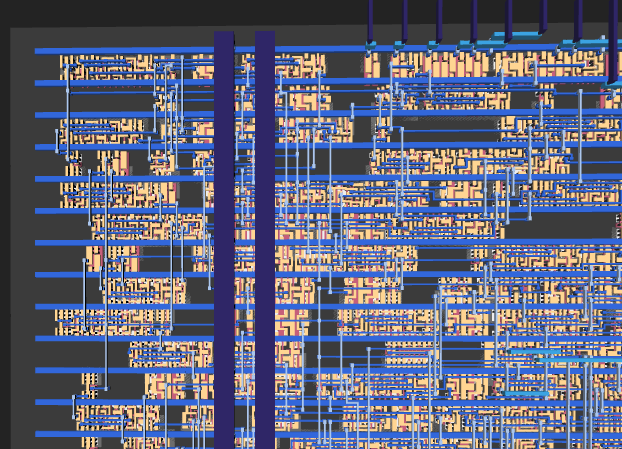
\includegraphics[width=\linewidth]{zoom_3d_sin_fill_decap.png}
  \caption{Sin celdas de relleno ni de desacople.}\label{fig:zoom_b}
\end{subfigure}

\vspace{6pt}
\begin{subfigure}[t]{0.48\textwidth}
  \centering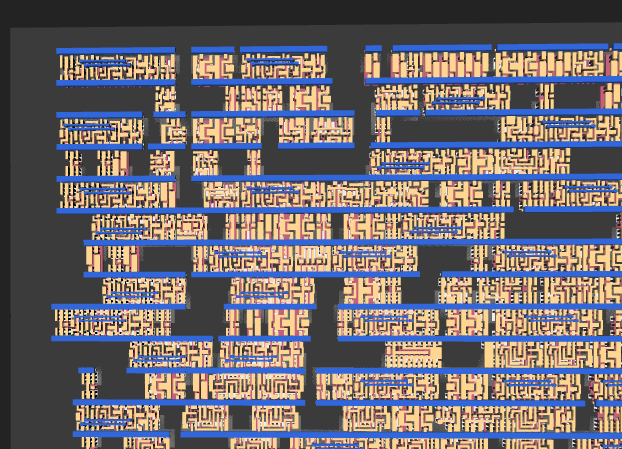
\includegraphics[width=\linewidth]{zoom_3d_celdas.png}
  \caption{Solo celdas estándar.}\label{fig:zoom_c}
\end{subfigure}\hfill
\begin{subfigure}[t]{0.48\textwidth}
  \centering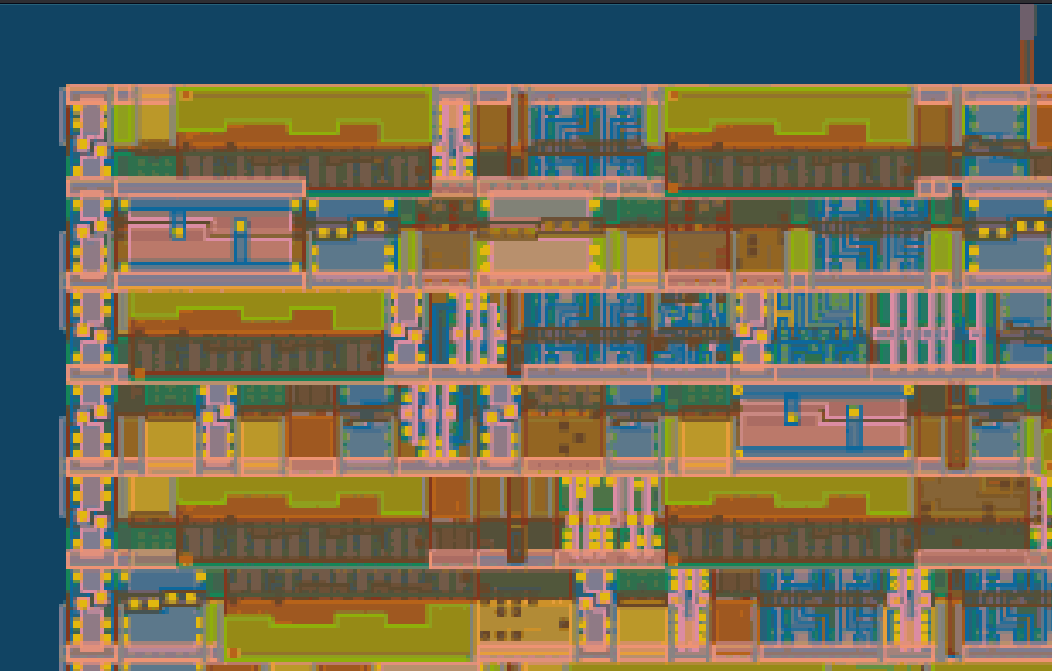
\includegraphics[width=\linewidth]{zoom_2d.png}
  \caption{Render 2D de la misma zona.}\label{fig:zoom_d}
\end{subfigure}
\caption{Ampliación de la esquina superior izquierda del diseño con distintas capas visibles.}
\label{fig:zoom}
\end{figure}

\begin{itemize}
  \item \textbf{Figura~\ref{fig:zoom_a}.} Las franjas azules horizontales son los rieles de alimentación (VPWR/VGND) en metal~1, uno por fila de celdas. Las dos bandas verticales moradas pertenecen al power grid en metal~4, y las líneas verticales delgadas son el ruteo de señales. En la parte superior se observan las conexiones de los pines.
  \item \textbf{Figura~\ref{fig:zoom_b}.} Al ocultar las celdas de relleno (\emph{fill}) y de desacople (\emph{decap}) aparecen huecos: esa área no contiene lógica. La densidad de colocación objetivo fue del 70\,\%.
  \item \textbf{Figura~\ref{fig:zoom_c}.} Sin el ruteo ni el power grid quedan solo las celdas estándar, alineadas en filas. Las franjas azules que permanecen son los rieles propios de cada celda.
  \item \textbf{Figura~\ref{fig:zoom_d}.} Vista plana con los colores de capa de sky130. En el borde izquierdo se observa la columna de celdas de borde de fila, y las celdas más anchas corresponden a elementos secuenciales (flip-flops).
\end{itemize}

\section{Corte lateral y vista oblicua}

La Figura~\ref{fig:corte} muestra el apilamiento vertical de capas en una sección aislada del diseño: en la parte inferior las regiones de difusión y pozos; encima, el polisilicio, los contactos, la capa de interconexión local (li1) y los metales. La Figura~\ref{fig:oblicua} muestra el diseño completo en perspectiva, donde se distinguen el power grid vertical y la densidad del ruteo.

\begin{figure}[htbp]
\centering
\begin{subfigure}[t]{0.44\textwidth}
  \centering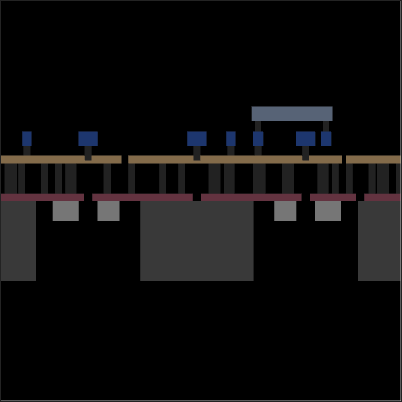
\includegraphics[width=\linewidth]{corte_lateral_3d.png}
  \caption{Corte lateral de una sección aislada.}\label{fig:corte}
\end{subfigure}\hfill
\begin{subfigure}[t]{0.50\textwidth}
  \centering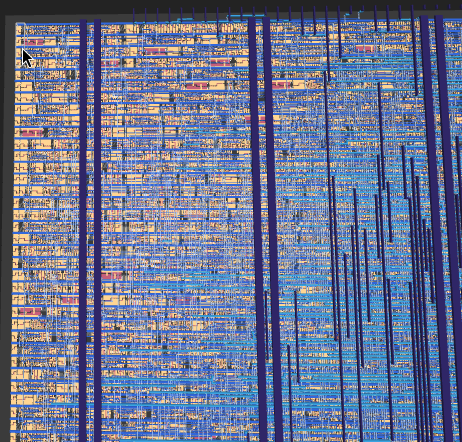
\includegraphics[width=\linewidth]{vista_oblicua_3d.png}
  \caption{Vista oblicua del diseño completo.}\label{fig:oblicua}
\end{subfigure}
\caption{Vistas 3D adicionales del layout.}
\end{figure}

\section{Resultados de implementación}

La Tabla~\ref{tab:metricas} recoge las métricas que reporta el flujo LibreLane en el archivo \code{stats/metrics.csv} del repositorio del shuttle~\cite{repo_shuttle}.

\begin{table}[htbp]
\centering
\caption{Resultados de implementación del diseño fabricado.}
\label{tab:metricas}
\begin{tabular}{>{\raggedright\arraybackslash}p{9.2cm} >{\raggedright\arraybackslash}p{4.8cm}}
\toprule
\textbf{Métrica} & \textbf{Valor} \\
\midrule
Utilización del área & 76,0\,\% \\
Área de celdas estándar & 113\,440\,\um$^2$ \\
Celdas secuenciales (flip-flops) & 1\,515 \\
Celdas combinacionales de varias entradas & 5\,758 \\
Buffers e inversores del árbol de reloj & 80 + 1\,296 \\
Buffers de reparación de tiempos & 2\,259 \\
Celdas de relleno / tap & 7\,159 / 2\,158 \\
Diodos de antena insertados & 122 \\
Errores de DRC de ruteo (final) & 0 (tras 7 iteraciones) \\
\midrule
Holgura de setup, esquina típica (tt, 25\,°C, 1,80\,V) & $+3{,}50$\,ns \\
Holgura de hold, esquina típica & $+0{,}31$\,ns \\
Holgura de setup, esquina lenta (ss, 100\,°C, 1,60\,V) & $-4{,}85$\,ns (peor caso) \\
\midrule
Potencia estimada, esquina típica & 6,58\,mW \\
\bottomrule
\end{tabular}
\end{table}

Antes del envío, el precheck de Tiny Tapeout aprobó todas sus verificaciones: Magic DRC, KLayout FEOL y BEOL, \emph{offgrid}, superposición de etiquetas de pines, áreas nulas, pines, límites, alimentación, capas, nombres de celdas, \emph{urpm/nwell} y pines analógicos.

\section{Observaciones}

\begin{itemize}
  \item Con la restricción de 25\,ns, el diseño cumple tiempos en las esquinas típica y rápida, pero no en la lenta (ss, 100\,°C): en el peor caso requeriría un periodo cercano a 30\,ns (unos 33\,MHz). Las pruebas de este documento se hicieron a 100\,kHz, muy por debajo de ese límite.
  \item LibreLane reporta 20 redes con violaciones de antena después de insertar los diodos; el precheck de Tiny Tapeout no las marcó como bloqueantes.
  \item La carpeta \code{tinytapeout\_femto\_UN/} del repositorio de la organización corresponde al commit \code{b28ff83}, posterior a la fabricación. Respecto al commit fabricado (\code{baab83f}) solo difiere el archivo \code{src/MappedSPIFlash.v}. El análisis de los capítulos siguientes se basa en el Verilog del commit fabricado.
\end{itemize}

% ======================================================================
\chapter{Montaje físico}
\label{cap:montaje}

\section{Equipos}

Todas las pruebas se hicieron con el mismo montaje, mostrado en las Figuras~\ref{fig:montaje_general} y~\ref{fig:montaje_detalle}. Participan cinco elementos conectados al mismo computador o alimentados desde él: la placa de demostración con el chip, el ESP32-C6 que hace de memoria flash, la memoria FM25V02, el adaptador USB-UART por el que se lee el chip y el analizador lógico que captura las señales.

\begin{figure}[htbp]
\centering
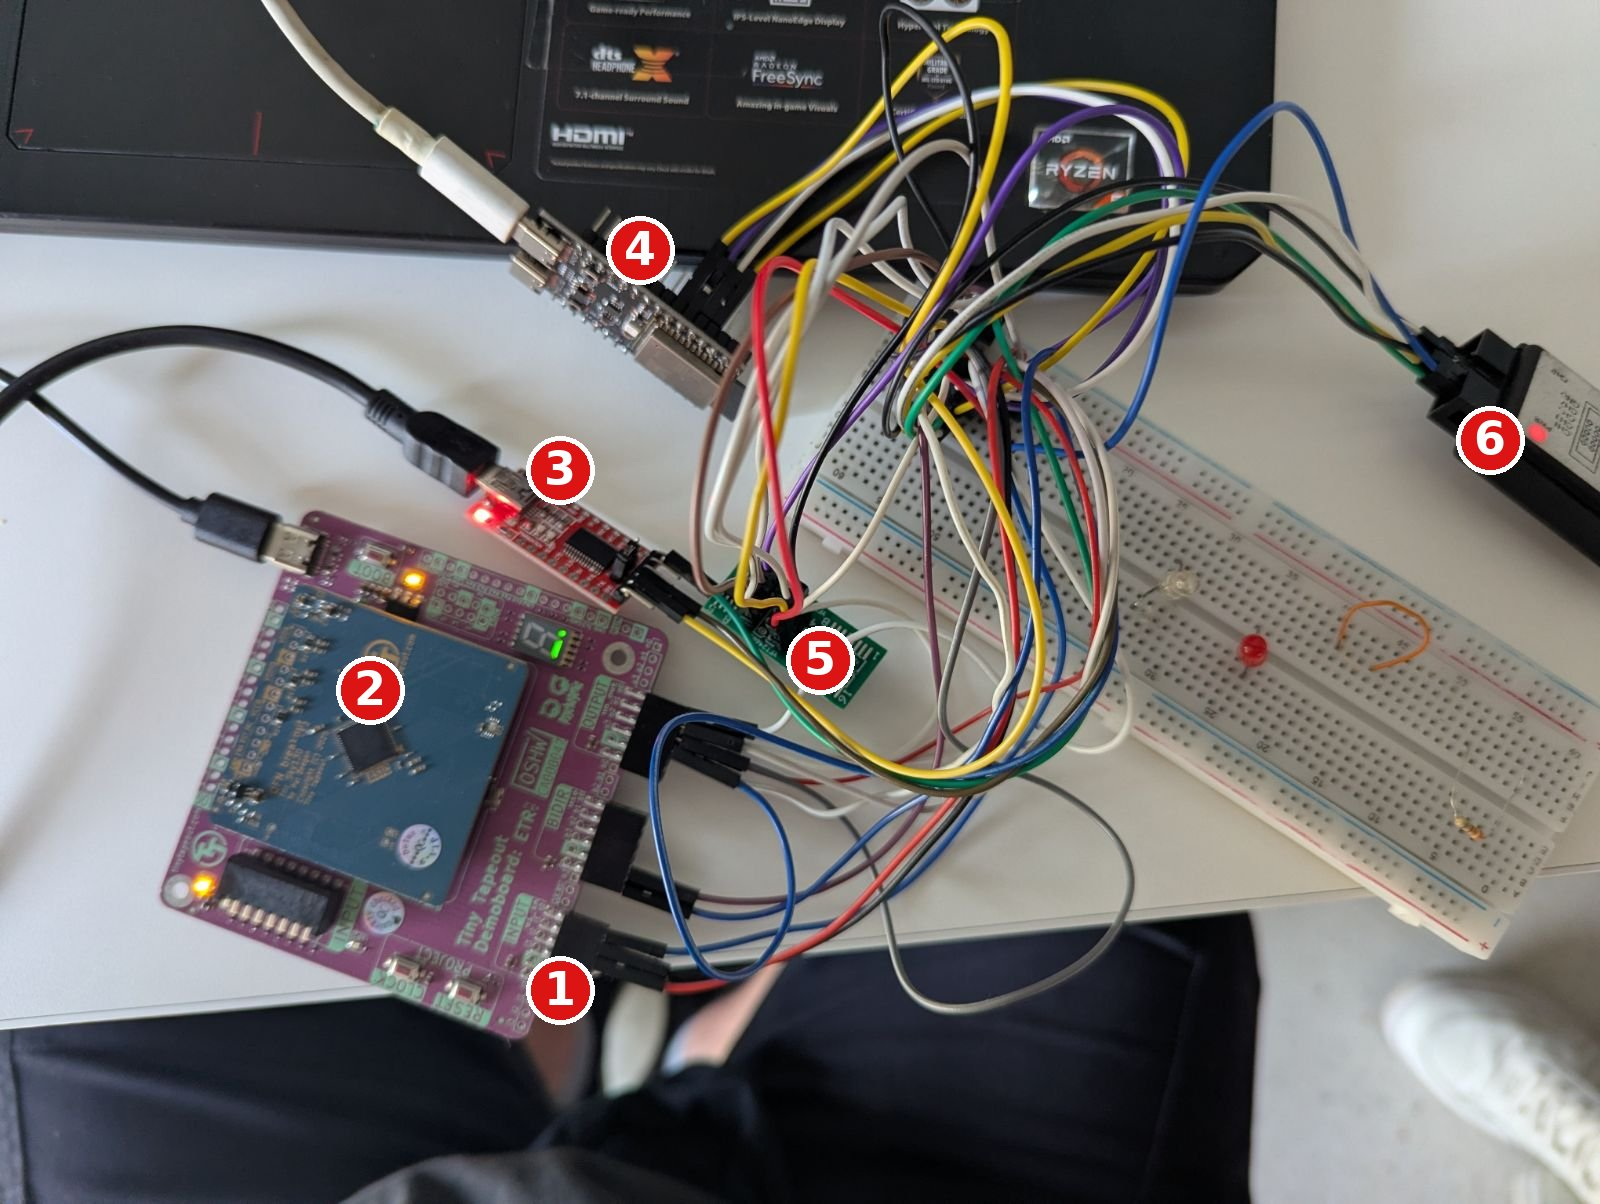
\includegraphics[width=0.92\textwidth]{montaje_general.jpg}
\caption{Montaje completo de las pruebas: (1) placa de demostración de Tiny Tapeout; (2) chip femto\_UN sobre la placa adaptadora QFN para sky130; (3) adaptador USB-UART FTDI; (4) ESP32-C6, memoria flash emulada; (5) memoria FM25V02 en su adaptador SOIC; (6) analizador lógico.}
\label{fig:montaje_general}
\end{figure}

\begin{figure}[htbp]
\centering
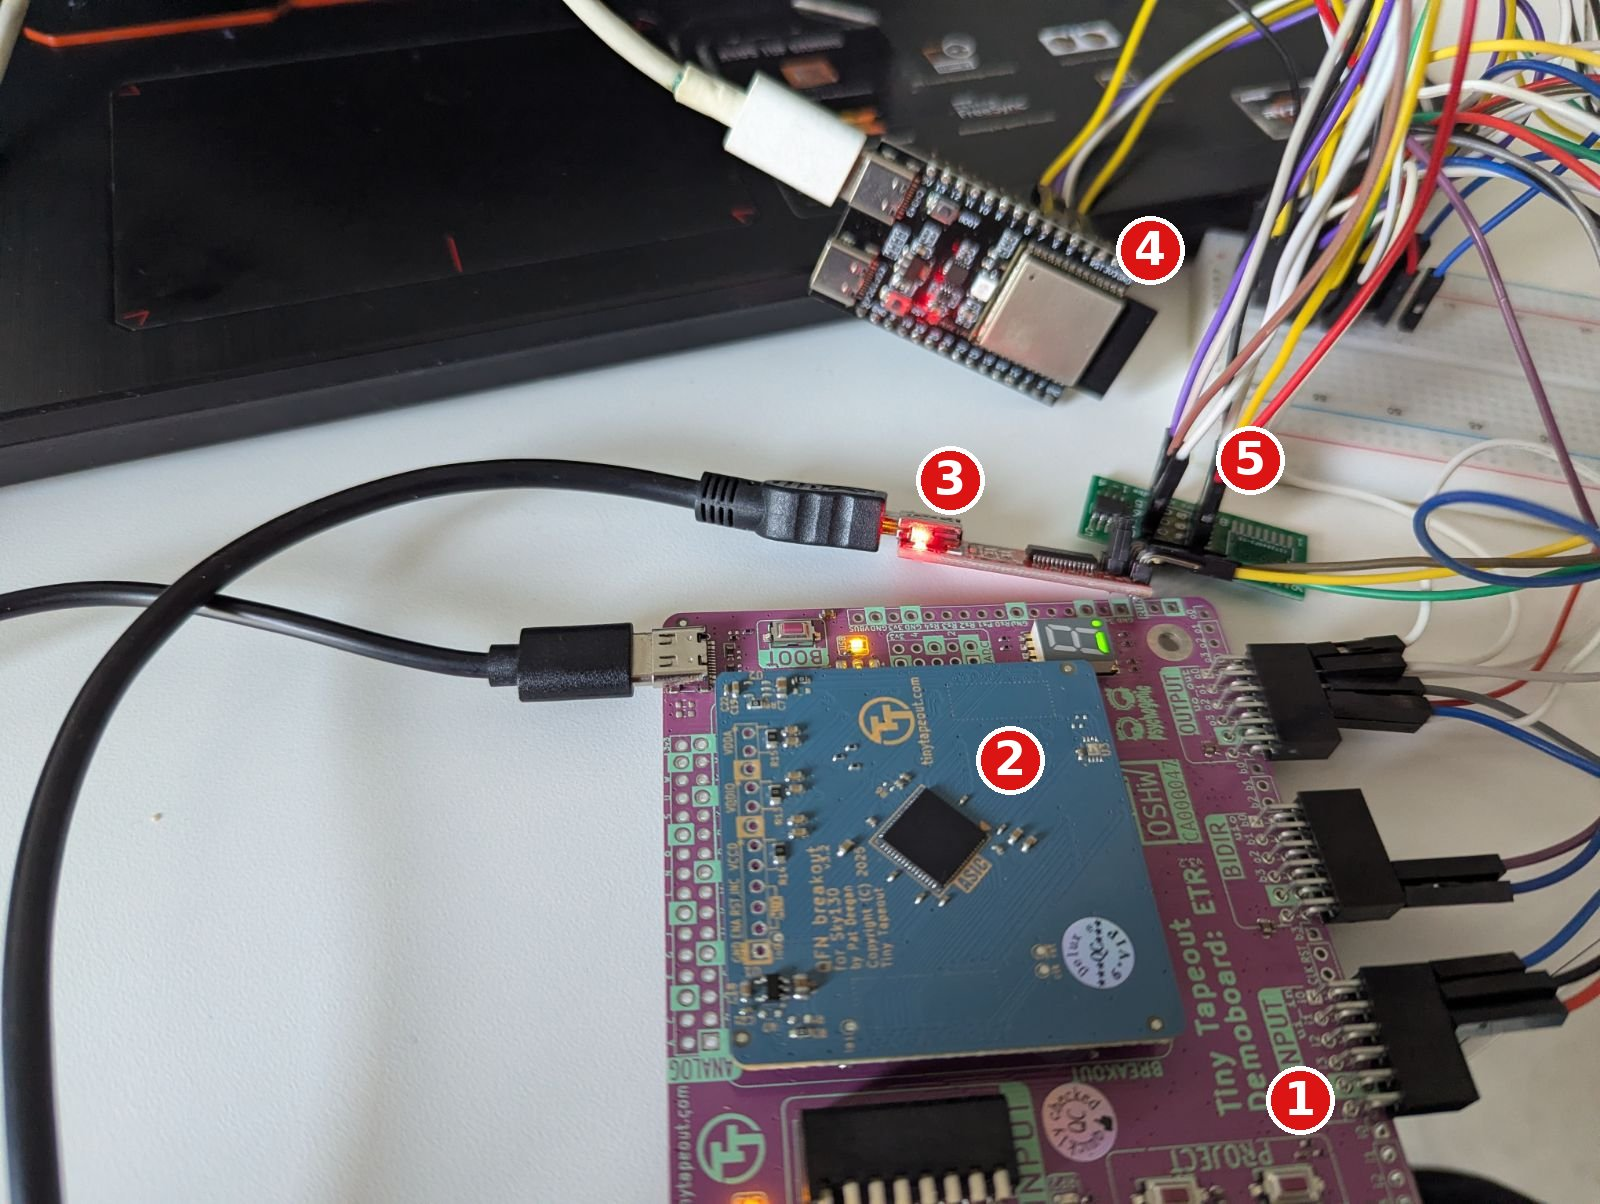
\includegraphics[width=0.92\textwidth]{montaje_detalle.jpg}
\caption{Detalle del montaje con la misma numeración de la Figura~\ref{fig:montaje_general}. Los cables salen de los conectores PMOD de entrada, salida y bidireccionales de la placa de demostración.}
\label{fig:montaje_detalle}
\end{figure}

\section{Conexiones}

La Tabla~\ref{tab:conexiones} reúne las conexiones de las tres interfaces del chip. Los pines se tomaron de la serigrafía de la placa de demostración y del archivo \code{info.yaml} del proyecto.

\begin{table}[htbp]
\centering
\caption{Conexiones del femto\_UN con la flash emulada, la RAM y la UART.}
\label{tab:conexiones}
{\small
\begin{tabular}{l l l l l}
\toprule
\textbf{Interfaz} & \textbf{Señal} & \textbf{Pin del chip} & \textbf{Destino} & \textbf{Pin del destino} \\
\midrule
Flash (ESP32-C6) & Selección (CS)      & \code{uo[2]} & ESP32-C6 & GPIO7 \\
                 & Reloj (CLK)         & \code{uo[5]} & ESP32-C6 & GPIO6 \\
                 & Datos a la memoria (MOSI) & \code{uo[0]} & ESP32-C6 & GPIO5 \\
                 & Datos al chip (MISO)& \code{ui[0]} & ESP32-C6 & GPIO4 \\
\midrule
RAM (FM25V02)    & Selección (CS)      & \code{uo[3]} & FM25V02 & CS \\
                 & Reloj (CLK)         & \code{uo[4]} & FM25V02 & SCK \\
                 & Datos a la memoria (MOSI) & \code{uo[1]} & FM25V02 & SI \\
                 & Datos al chip (MISO)& \code{ui[1]} & FM25V02 & SO \\
                 & Alimentación        & 3,3\,V       & FM25V02 & VDD \\
\midrule
UART (FTDI)      & Transmisión (TXD)   & \code{uo[7]} & USB-UART & RXD \\
                 & Recepción (RXD)     & \code{ui[2]} & USB-UART & TXD \\
\midrule
Todas            & Tierra              & GND          & Todos    & GND \\
\bottomrule
\end{tabular}
}
\end{table}

\section{Condiciones del montaje}

Cuatro condiciones resultaron necesarias para que el montaje funcione:

\begin{itemize}
  \item Los ocho interruptores DIP de la placa de demostración deben estar apagados; encendidos, fuerzan las entradas del chip.
  \item No se unen los 3,3\,V de la placa de demostración y del ESP32-C6. Cada una se alimenta por su USB y solo comparten tierra. La FM25V02 se alimenta de los 3,3\,V de la placa de demostración.
  \item La placa de demostración se conecta primero y el ESP32-C6 después. En el orden contrario, la placa de demostración arrancó en modo de carga de firmware.
  \item El archivo \code{femto\_setup.py} de la placa de demostración selecciona el proyecto \code{tt\_um\_femto} y deja como entradas del RP2040 los pines que manejan la flash, la RAM y la UART, para no entrar en conflicto con ellos.
\end{itemize}

% ======================================================================
\chapter{ESP32-C6 como memoria flash y primer arranque}
\label{cap:flash}

\section{Propósito}

Este capítulo describe la prueba con la que el femto\_UN ejecutó su primer programa en hardware: arrancar desde una memoria de programa y enviar el mensaje \code{Hello World from femto UN} por la UART.

La memoria de programa no es un chip de flash, sino un ESP32-C6 programado para comportarse como una flash SPI de solo lectura. El capítulo explica por qué se llegó a esa solución, cómo funciona el emulador, qué se aprendió del bus SPI del chip al hacerlo funcionar y el resultado obtenido. El material está en dos carpetas del repositorio: \href{\repo/firmware/esp32_flash_emu}{firmware/esp32\_flash\_emu}, con el programa del ESP32, y \href{\repo/asic/hello_world_uart}{asic/hello\_world\_uart}, con la prueba completa.

\section{Por qué un ESP32 como memoria}

El plan inicial era usar un módulo comercial de flash SPI, grabado con un programador CH341A. Ese módulo resultó no ser confiable por dos razones:

\begin{itemize}
  \item El programa \code{flashrom} lo identificó como una W25Q64.W, con identificador \code{EF 60 17}. Esa familia trabaja a 1,8\,V, no a los 3,3\,V del chip.
  \item Al medirlo, su pin de salida de datos estaba en corto con tierra, de modo que el procesador siempre leía ceros.
\end{itemize}

Con un ESP32-C6 disponible, se optó por programarlo para que respondiera como una flash. Además de reemplazar el módulo, esta solución dio una ventaja que un chip real no ofrece: el emulador registra cada transacción que recibe, y eso permitió ver qué le pedía exactamente el procesador.

\section{El emulador de flash}

El programa del ESP32 está en \code{esp32\_flash\_emu.ino}. Su comportamiento es el de una flash SPI en modo~0, limitada a la lectura:

\begin{enumerate}
  \item Espera a que la línea de selección baje.
  \item Lee los ocho bits del comando, uno en cada flanco de subida del reloj.
  \item Si el comando es de lectura (\code{0x03}), lee los 24 bits de dirección y entrega los bytes del programa, uno tras otro, mientras la línea de selección siga en bajo.
  \item Si el comando es cualquier otro, lo ignora y deja la línea de datos en alto.
  \item Cuando la línea de selección sube, vuelve a dejar la línea de datos en alto y espera la siguiente transacción.
\end{enumerate}

Las direcciones que quedan fuera del programa devuelven \code{FF}, como una flash borrada. El punto~4 es la parte central del emulador y corresponde a este fragmento:

\begin{lstlisting}
// Solo responde a READ (0x03). Cualquier otra cosa se ignora
// y MISO queda en alto.
if (bits != 0x03) { logit(bits, 3, 0, 0); return; }
\end{lstlisting}

El programa del procesador se incluye en el emulador como un arreglo de bytes, generado a partir del archivo binario con \code{xxd -i}, y queda en \code{firmware.h}.

\subsection{Atención del bus por software}

El emulador no usa el periférico SPI del ESP32. Lee y escribe los pines directamente desde un bucle, consultando el registro de entradas del microcontrolador. Esto da control total sobre el momento en que se muestrea cada línea, que es lo que permitió ajustarlo al comportamiento particular del chip, pero limita la velocidad: funciona con el reloj del procesador en 100\,kHz, lo que da un reloj SPI de unos 33\,kHz, y no a los 24\,MHz para los que se diseñó el chip.

\subsection{Registro de transacciones}

El emulador guarda las últimas 32 transacciones con su comando, su dirección y la cantidad de bytes enviados. Con el procesador en reset, al escribir \code{p} en el monitor serie imprime ese registro, y con \code{c} lo borra. Cada transacción queda clasificada como lectura atendida, comando ignorado o transacción incompleta. Mientras el procesador corre, el emulador no atiende el monitor serie, para no perder flancos del reloj.

\section{Comportamiento del bus SPI del chip}

Para que el emulador funcionara hubo que entender cómo lee la memoria el chip fabricado. Lo que sigue sale de leer el Verilog que se envió a fabricar (commit \code{baab83f} del repositorio \code{cicamargoba/femto\_UN}) y de las capturas del analizador lógico.

\subsection{El reloj SPI nunca se detiene}

El reloj SPI del chip es el reloj del sistema dividido entre tres, y sigue corriendo aunque no haya ninguna lectura en curso. Está en alto durante un ciclo del reloj del sistema y en bajo durante dos. Cada lectura ocupa 65 períodos del reloj SPI: 32 para el comando y la dirección y 33 para los datos.

Además, el chip muestrea la línea de datos un bit tarde. Por esa razón el programa no se graba tal como lo produce el compilador, sino corrido un bit a la derecha. El archivo que se carga en la memoria es \code{firmware\_shifted.bin}, generado por el propio proceso de compilación.

\subsection{Las tres fases de la línea de selección}

Como el reloj no se detiene, la línea de selección puede bajar en tres momentos distintos respecto al reloj, según la instrucción que el procesador acaba de ejecutar. La Tabla~\ref{tab:fases} describe cada caso.

\begin{table}[htbp]
\centering
\caption{Fases de la línea de selección respecto al reloj SPI.}
\label{tab:fases}
\begin{tabular}{c >{\raggedright\arraybackslash}p{5.6cm} >{\raggedright\arraybackslash}p{7.4cm}}
\toprule
\textbf{Fase} & \textbf{Cuándo ocurre} & \textbf{Qué recibe la memoria} \\
\midrule
0 & Lectura de instrucción después de una instrucción normal & La selección baja un ciclo antes del primer flanco: comando \code{03} correcto \\
1 & Lectura de instrucción después de un acceso a la UART & La selección baja a la vez que sube el reloj; funciona si la memoria alcanza a ver ese flanco \\
2 & Carga de datos desde la flash, la lectura siguiente y las dos primeras lecturas tras el reset & El primer bit del comando no llega: la memoria recibe \code{06} y no responde \\
\bottomrule
\end{tabular}
\end{table}

La Figura~\ref{fig:fase2zoom} muestra la fase~2 ampliada. La línea de selección sube y baja junto con un pulso del reloj, entre 1940\,µs y 1950\,µs, que es un ciclo del reloj del sistema a 100\,kHz. Ese pulso ocurre con la selección en alto, así que la memoria no lo cuenta, y el comando empieza un bit tarde: en la línea MOSI se decodifica \code{06} en lugar de \code{03}.

\begin{figure}[htbp]
\centering
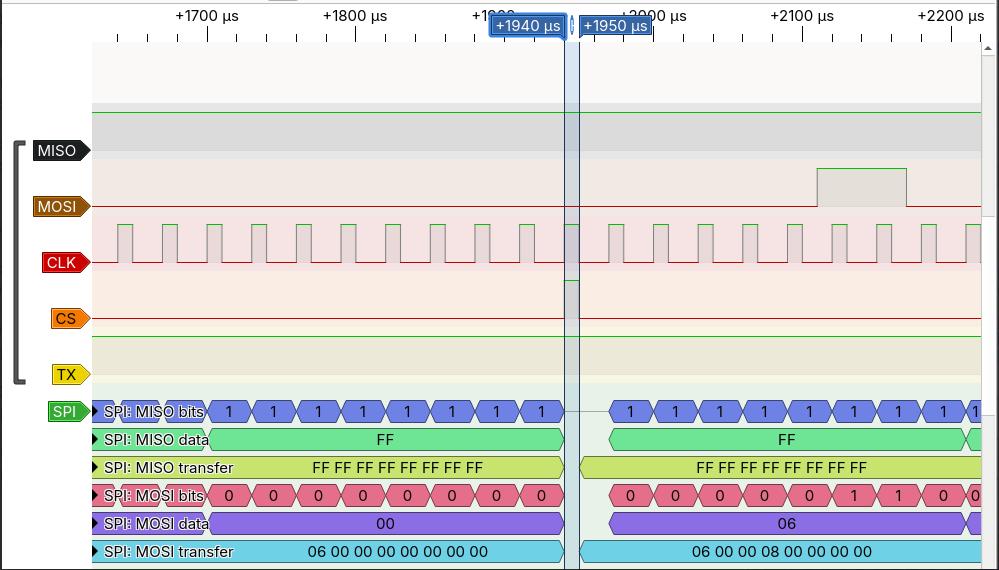
\includegraphics[width=0.95\textwidth]{flash_fase2_zoom.png}
\caption{Fase~2: la línea de selección conmuta junto con un pulso del reloj, entre 1940\,µs y 1950\,µs.}
\label{fig:fase2zoom}
\end{figure}

La Figura~\ref{fig:fase2ms} confirma la cuenta. Entre un pulso de la línea de selección y el siguiente hay 1,89\,ms, que a 33\,kHz corresponden a 64 flancos de subida: uno menos que los 65 que necesita una lectura completa.

\begin{figure}[htbp]
\centering
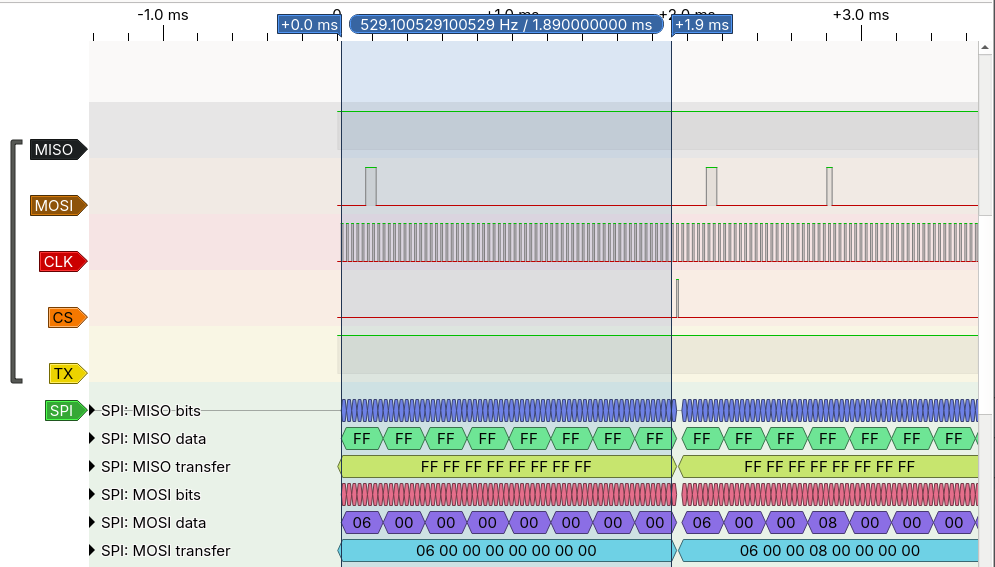
\includegraphics[width=0.95\textwidth]{flash_fase2_189ms.png}
\caption{Lectura en fase~2: 64 flancos de subida entre dos pulsos de la línea de selección (1,89\,ms).}
\label{fig:fase2ms}
\end{figure}

El valor \code{06} corresponde, en una flash real, al comando de habilitación de escritura. Aquí nadie está escribiendo: es el comando de lectura visto con un bit de corrimiento.

\subsection{El arranque depende del nivel de la línea de datos}

Después del reset, las dos primeras lecturas salen en fase~2 y la memoria las ignora. Lo que pasa a continuación depende del nivel en que queda la línea MISO cuando la memoria no responde:

\begin{itemize}
  \item \textbf{MISO en alto.} El procesador lee \code{FFFFFFFF}. Su decodificador interpreta ese valor como un salto de dos bytes hacia atrás, con lo que vuelve a la dirección~0, esta vez en fase~0, y arranca correctamente.
  \item \textbf{MISO en bajo.} El procesador lee \code{00000000}, que corresponde a una carga de datos desde la flash. Esa carga produce otra lectura en fase~2, que devuelve otro cero, y el procesador queda pidiendo la dirección~0 indefinidamente.
\end{itemize}

De aquí salen las dos condiciones que debe cumplir cualquier memoria conectada a este chip: \textbf{ignorar los comandos que no sean de lectura} y \textbf{dejar la línea MISO en alto cuando está en reposo}.

La Figura~\ref{fig:arranque} muestra el arranque completo. Las dos primeras transacciones llegan como \code{06 00 00 00} y \code{06 00 00 08}, que son las lecturas de las direcciones~0 y~4 con el primer bit perdido, y la memoria no contesta: MISO permanece en \code{FF}. La tercera es \code{03 00 00 00}, de nuevo desde la dirección~0, y la memoria entrega \code{1B 81 A0 00}, los primeros bytes del programa.

\begin{figure}[htbp]
\centering
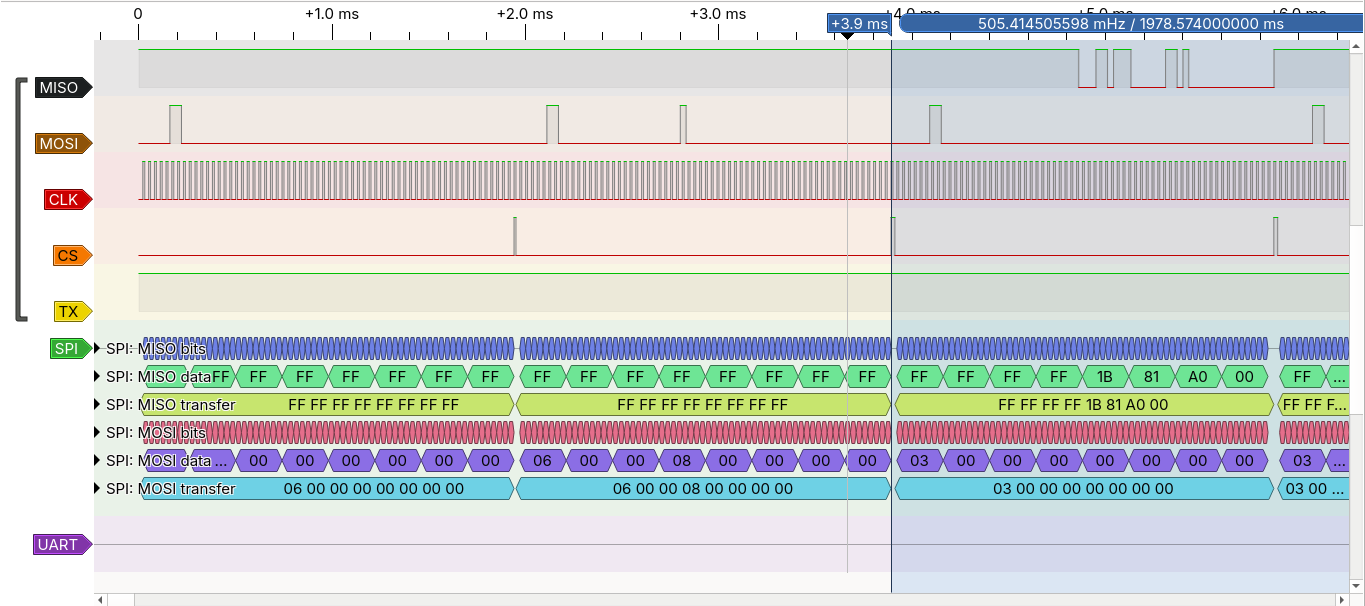
\includegraphics[width=\textwidth]{flash_arranque.png}
\caption{Arranque del femto\_UN: dos lecturas ignoradas (\code{06 \ldots}) y reinicio desde la dirección~0 con \code{03 00 00 00}.}
\label{fig:arranque}
\end{figure}

\subsection{Velocidad de la UART}

El divisor de la UART está fijo dentro del chip. Según el Verilog, cada bit dura 208 ciclos del reloj del sistema, de modo que la velocidad es
\[
\text{velocidad} = \frac{f_\text{reloj}}{208}.
\]
Con el reloj en 100\,kHz resultan 481 baudios. El valor se comprobó en el analizador lógico: nueve bits ocupan cerca de 18,7\,ms.

\section{Procedimiento}

\begin{enumerate}
  \item \textbf{Compilar el programa del procesador.} Se usa el programa \code{uart\_full\_demo.S} del repositorio del femto\_UN, compilado con \code{riscv-none-elf-gcc}. El proceso genera \code{firmware\_shifted.bin}, de 1120 bytes.
  \item \textbf{Cargar el emulador en el ESP32-C6.} Se convierte el binario a \code{firmware.h} y se compila y carga con \code{arduino-cli}.
  \item \textbf{Configurar la placa de demostración.} El archivo \code{femto\_setup.py} se copia a la placa con \code{mpremote}. Este archivo selecciona el proyecto \code{tt\_um\_femto}, libera los pines que usan la flash, la RAM y la UART, pone el reloj a la frecuencia pedida y deja el chip en reset.
  \item \textbf{Abrir la UART.} En una terminal se abre \code{minicom} a 481 baudios sobre el adaptador USB-UART.
  \item \textbf{Soltar el reset.} En otra terminal, desde la consola de la placa de demostración, se ejecuta la configuración y se libera el reset.
\end{enumerate}

Los comandos de los dos últimos pasos son:

\begin{lstlisting}
sudo minicom -b 481 -D /dev/ttyUSB0

mpremote connect /dev/ttyACM0
>>> FREQ=100000; exec(open('femto_setup.py').read())
>>> tt.reset_project(False)
\end{lstlisting}

El procedimiento completo, con todos los comandos, está en el README de la prueba.

\section{Resultado}

Cerca de un segundo después de soltar el reset aparece el mensaje en \code{minicom}, como se ve en la Figura~\ref{fig:hello_minicom}. En la consola de la placa de demostración aparecen avisos de posible conflicto en \code{ui\_in0} a \code{ui\_in2}: son las líneas que manejan el ESP32 y el adaptador USB-UART, y por eso la configuración las deja como entradas.

\begin{figure}[htbp]
\centering
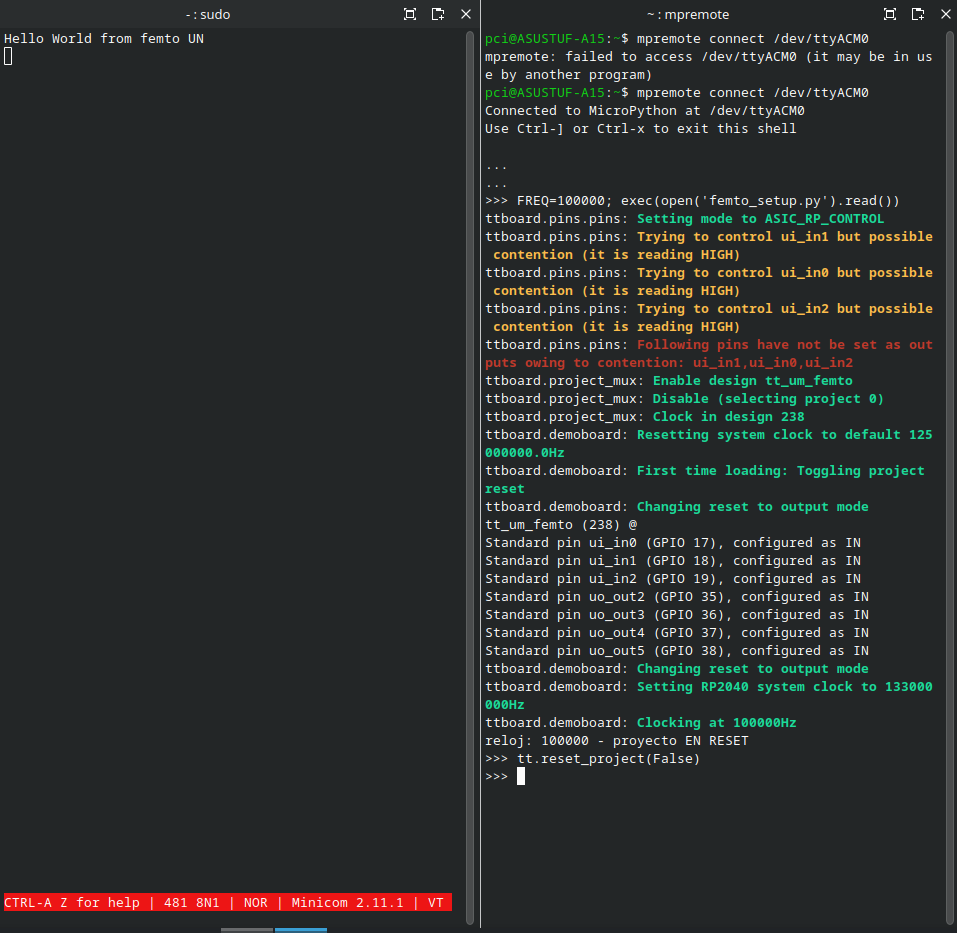
\includegraphics[width=0.62\textwidth]{hello_minicom.png}
\caption{Mensaje recibido en \code{minicom} (izquierda) y configuración de la placa de demostración desde \code{mpremote} (derecha).}
\label{fig:hello_minicom}
\end{figure}

La Figura~\ref{fig:hello_pv} muestra la misma prueba en el analizador lógico. El decodificador de UART a 481 baudios lee el mensaje carácter por carácter en la línea TX, mientras el bus SPI no deja de leer instrucciones. La Figura~\ref{fig:hello_pv_uart} amplía la decodificación de la UART con el mensaje completo.

\begin{figure}[htbp]
\centering
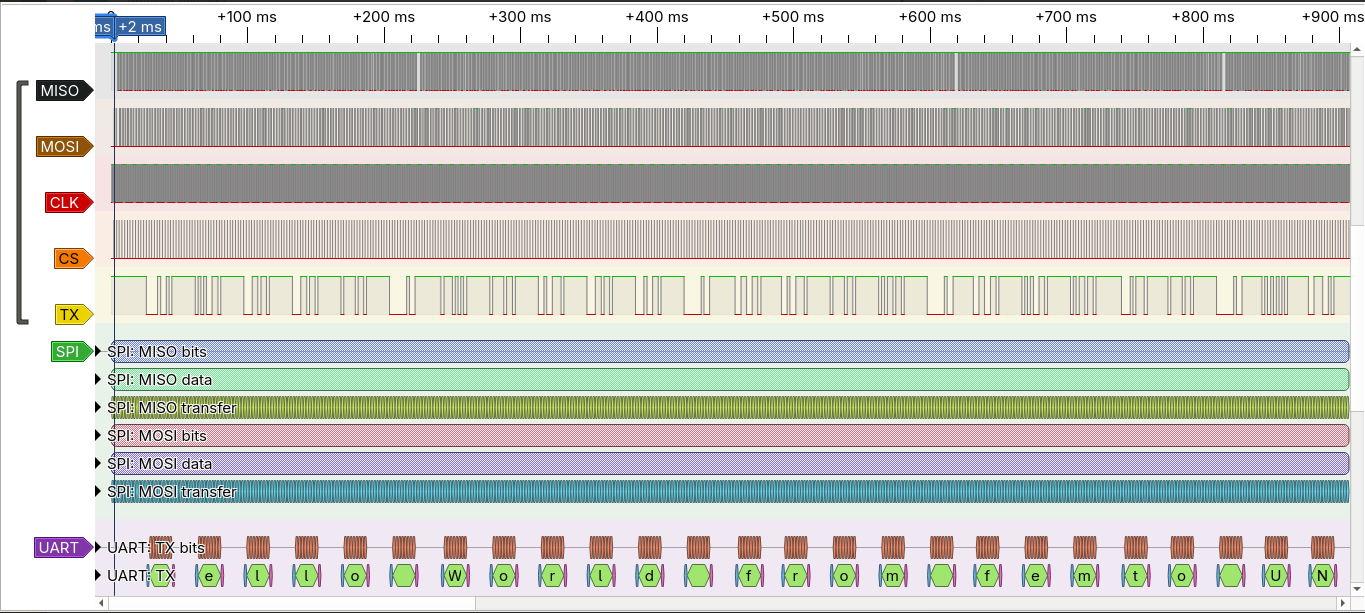
\includegraphics[width=\textwidth]{hello_pulseview.png}
\caption{Mensaje decodificado en PulseView junto con la actividad del bus SPI de la flash.}
\label{fig:hello_pv}
\end{figure}

\begin{figure}[htbp]
\centering
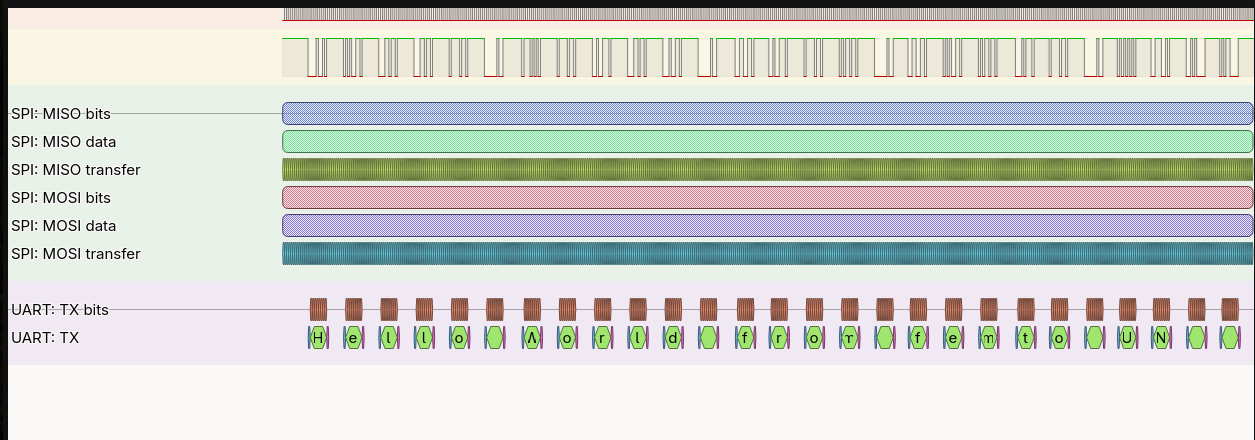
\includegraphics[width=\textwidth]{hello_pulseview_uart.png}
\caption{Decodificación de la UART: \code{Hello World from femto UN}.}
\label{fig:hello_pv_uart}
\end{figure}

La captura completa de PulseView (\code{ESP\_32\_FLASH\_TX}, 2\,s a 1\,MHz) se analizó también fuera de PulseView. En ella hay 1010 transacciones en el bus de la flash: 822 lecturas atendidas (\code{03}) y 187 que llegan como \code{06} y la memoria ignora. La decodificación de la línea TX a 481 baudios devuelve los 27 bytes del mensaje, \code{Hello World from femto UN} seguido del salto de línea, entre los 25,7\,ms y los 946,5\,ms de la captura.

Después del mensaje, el programa queda en un bucle de espera. Su retardo está calibrado para 24\,MHz, así que a 100\,kHz cada vuelta del bucle dura unos dos minutos.

\section{Problemas encontrados}

La Tabla~\ref{tab:problemas_flash} recoge los problemas que aparecieron durante la prueba.

{\small
\begin{longtable}{>{\raggedright\arraybackslash}p{4.4cm} >{\raggedright\arraybackslash}p{5cm} >{\raggedright\arraybackslash}p{5cm}}
\caption{Problemas encontrados durante el arranque del femto\_UN.}\label{tab:problemas_flash}\\
\toprule
\textbf{Síntoma} & \textbf{Causa} & \textbf{Solución} \\
\midrule
\endfirsthead
\toprule
\textbf{Síntoma} & \textbf{Causa} & \textbf{Solución} \\
\midrule
\endhead
Con la flash real, MISO siempre en 0 y el procesador repite \code{06 00 00 00} & MISO en bajo en reposo: el procesador queda en el bucle de cargas & Dejar MISO en alto en reposo \\
\code{ui[0]} forzado en 0 & La placa de demostración seguía manejando el pin como salida & Asignar el modo de entrada con \code{.mode = Pin.IN} \\
Entradas leyendo en alto y aviso de conflicto & Interruptores DIP encendidos & Todos apagados \\
La UART envía 27 bytes \code{00} en lugar del texto & El emulador contestaba también los comandos \code{06} y el procesador no reiniciaba & El emulador solo responde a \code{03} \\
\code{minicom} no muestra nada a 481 baudios & Los bytes eran \code{00}, que no se ven en pantalla & Medir el ancho de bit con el analizador \\
Con la punta del analizador en MISO, la línea no sube & La punta carga la línea hacia abajo & Medir sin esa punta, o manejar MISO con el ESP32 \\
La placa de demostración arranca en modo de carga & El ESP32 se conectó primero & Conectar primero la placa de demostración \\
No aparece el puerto del adaptador USB-UART & Falta el controlador & \code{sudo modprobe ftdi\_sio} \\
El ESP32 se reinicia por el watchdog & El emulador desactivaba las interrupciones con la selección atascada en bajo & Se quitó esa desactivación \\
\bottomrule
\end{longtable}
}

\section{Verificación con un modelo}

Para confirmar la explicación del arranque se escribió un modelo en Python, \code{sim\_femto.py}, que reproduce ciclo a ciclo el controlador de flash, el procesador y la UART del chip, y ejecuta el mismo programa. No es una simulación del Verilog, pero reproduce lo medido. La Tabla~\ref{tab:modelo} muestra lo que predice según cómo se comporte la memoria.

\begin{table}[htbp]
\centering
\caption{Salida de la UART según el comportamiento de la memoria, de acuerdo con el modelo.}
\label{tab:modelo}
\begin{tabular}{>{\raggedright\arraybackslash}p{7.4cm} >{\raggedright\arraybackslash}p{6.6cm}}
\toprule
\textbf{Comportamiento de la memoria} & \textbf{Salida por la UART} \\
\midrule
Contesta también los comandos \code{06} & 27 bytes \code{00}, uno cada 3564 ciclos \\
Solo contesta \code{03} y ve el flanco de la fase~1 & \code{Hello World from femto UN} \\
Solo contesta \code{03} y no ve el flanco de la fase~1 & La letra \code{H} repetida sin parar \\
\bottomrule
\end{tabular}
\end{table}

El primer caso coincide con lo observado en hardware antes de corregir el emulador: 3564 ciclos a 100\,kHz son 35,6\,ms, y entre bytes se midieron cerca de 35,5\,ms. El segundo es el resultado final. El tercero no se ha visto en hardware; es una predicción del modelo que indica qué buscar si otra memoria llega a fallar.

\section{Limitaciones}

\begin{itemize}
  \item El ESP32-C6 queda como la memoria de programa de las pruebas. El módulo de flash no sirvió y no se volverá a usar.
  \item Por esa razón las pruebas corren a 100\,kHz: el ESP32 atiende el bus por software y no alcanza el rango de 22,5 a 25\,MHz para el que se diseñó el chip. El comportamiento del procesador a esa velocidad queda sin comprobar.
  \item Las cargas de datos desde la flash no funcionan en este chip. El programa de demostración las evita usando valores inmediatos.
\end{itemize}

% ======================================================================
\chapter{Prueba de la memoria RAM SPI}
\label{cap:ram}

\section{Propósito}

Con el procesador arrancando desde el ESP32-C6, quedaba por probar el segundo bus SPI del chip: el de la memoria RAM. Este capítulo describe dos programas que se ejecutaron en el femto\_UN para comprobarlo. El primero lee y escribe posiciones fijas de la RAM e imprime los valores por la UART. El segundo usa la RAM como almacenamiento real: recibe texto por la UART, lo guarda en la memoria y lo devuelve en mayúsculas.

En el camino apareció un problema que no tiene solución en el hardware: el controlador de RAM del chip no envía el comando que la memoria exige antes de cada escritura. El capítulo explica cómo se resolvió desde el programa, aprovechando el mismo defecto de sincronización del reloj SPI descrito en el Capítulo~\ref{cap:flash}.

Todo se hizo con el montaje del Capítulo~\ref{cap:montaje}: el ESP32-C6 como memoria de programa, el reloj del procesador en 100\,kHz y la UART a 481 baudios.

\section{La memoria FM25V02}

La FM25V02 es una memoria ferroeléctrica (F-RAM) de 256\,kbit, es decir 32\,KB, con interfaz SPI y alimentación de 3,3\,V. Se lee y se escribe como una RAM, byte a byte y sin tiempos de espera, pero a diferencia de una RAM convencional conserva los datos sin alimentación. Esa propiedad se aprovechó para comprobar que las escrituras realmente llegan a la memoria.

Antes de conectarla al procesador, la memoria se probó sola con el ESP32-C6, que leyó su identificador (\code{C2 22 00}) y recorrió los 32\,KB sin errores. En esa prueba quedaron grabados algunos datos que el primer programa de este capítulo vuelve a leer. La Tabla~\ref{tab:comandos} muestra los comandos de la memoria que intervienen en este capítulo.

\begin{table}[htbp]
\centering
\caption{Comandos de la FM25V02 que intervienen en la prueba.}
\label{tab:comandos}
\begin{tabular}{c c l}
\toprule
\textbf{Código} & \textbf{Comando} & \textbf{Función} \\
\midrule
\code{03} & READ & Leer desde una dirección \\
\code{02} & WRITE & Escribir desde una dirección \\
\code{06} & WREN & Habilitar la escritura \\
\code{04} & WRDI & Deshabilitar la escritura \\
\bottomrule
\end{tabular}
\end{table}

La memoria solo acepta un WRITE si antes recibió un WREN, y cada escritura completada vuelve a deshabilitarla. Es decir, cada escritura necesita su propio WREN.

\section{Montaje}

La FM25V02 se montó en un adaptador SOIC, elemento~5 de la Figura~\ref{fig:montaje_general}, y se conectó a los pines del chip indicados en la Tabla~\ref{tab:conexiones}. El archivo \code{femto\_setup.py} ya libera los pines \code{ui[1]}, \code{uo[3]} y \code{uo[4]}, así que no hubo que cambiar la configuración de la placa de demostración.

\section{El bus de la RAM en el chip}

\subsection{Reloj y fases}

El bus de la RAM se comporta como el de la flash, con un reloj más lento. Su reloj es el del sistema dividido entre 11, unos 9,1\,kHz con el procesador a 100\,kHz ---el mismo valor que se mide en las capturas---, y tampoco se detiene nunca. Por eso la línea de selección puede bajar en cualquiera de las 11 posiciones posibles respecto a ese reloj, que aquí se llaman fases. Si baja con el reloj en alto, la memoria pierde el primer bit del comando, igual que ocurre con la flash.

La consecuencia sobre los dos comandos que envía el controlador es directa:

\begin{itemize}
  \item Una lectura (\code{03}, en binario \code{0000 0011}) llega como \code{06} (\code{0000 0110}): la memoria la toma como WREN.
  \item Una escritura (\code{02}, \code{0000 0010}) llega como \code{04} (\code{0000 0100}): la memoria la toma como WRDI.
\end{itemize}

Otros dos detalles del controlador, tomados del código de prueba, afectan a los programas: solo usa los bits 15 a 8 de la dirección, y el bit~31 de cada palabra leída no es válido, por lo que los programas lo descartan.

\subsection{El controlador no envía WREN}

El controlador de RAM del chip solo envía READ y WRITE; nunca envía WREN. Como la FM25V02 rechaza cualquier escritura que no venga precedida de un WREN, con un acceso normal ninguna escritura llega a la memoria.

La solución sale del defecto anterior. Si justo antes de cada escritura el programa hace una lectura cuya línea de selección baja en una fase mala, la memoria recibe \code{06}, que es exactamente el WREN que hace falta. La escritura siguiente, en fase buena, llega como un WRITE válido. En el código esa lectura aparece así:

\begin{lstlisting}
    PAD 6
    lw t0, 0(s8)   # A PROPOSITO en fase mala: la F-RAM recibe 06 = WREN
    PAD 7
    sw s6, 0(s8)   # escritura
\end{lstlisting}

\subsection{Cómo se controla la fase desde el programa}

Para que la lectura que hace de WREN caiga en fase mala y todos los demás accesos en fase buena, el programa tiene que saber en qué fase está el reloj de la RAM en cada acceso. Según los comentarios del código:

\begin{itemize}
  \item Una instrucción normal tarda 198 ciclos de reloj, que es múltiplo de 11, así que por sí sola no cambia la fase. La UART tampoco la cambia; solo la cambian los accesos a la RAM.
  \item La instrucción \code{slli zero, zero, 2} no hace nada útil, pero tarda 201 ciclos y adelanta la fase 3 posiciones.
\end{itemize}

Con eso se define una macro, \code{PAD n}, que inserta $n$ de esas instrucciones antes de un acceso. Los valores de cada \code{PAD} se obtuvieron con el modelo ciclo a ciclo del chip, de modo que los accesos normales caen en fase~0 (la selección baja 5 ciclos antes de un flanco de subida) y la lectura que hace de WREN cae en fase~8.

Este ajuste es frágil: si se agrega, quita o reordena un acceso a la RAM, hay que volver a calcular todos los \code{PAD}.

\section{Prueba de lectura, escritura y persistencia}

\subsection{El programa}

El programa \code{ram\_test.S} imprime un encabezado y cuatro líneas, descritas en la Tabla~\ref{tab:lineas}, y termina con \code{FIN}.

\begin{table}[htbp]
\centering
\caption{Líneas que imprime \code{ram\_test.S}.}
\label{tab:lineas}
\begin{tabular}{c l >{\raggedright\arraybackslash}p{9cm}}
\toprule
\textbf{Línea} & \textbf{Posición} & \textbf{Qué hace} \\
\midrule
L1 & RAM + \code{0x0000} & Lee la posición e imprime su valor \\
L2 & RAM + \code{0x1000} & Igual que L1, en otra posición \\
E1 & RAM + \code{0x2000} & Lee un contador, le suma 1, lo escribe con el WREN provocado y lo relee. Imprime el valor anterior y el releído \\
E2 & RAM + \code{0x3000} & Lo mismo, pero sin el WREN provocado. Es la prueba de control \\
\bottomrule
\end{tabular}
\end{table}

La rutina que imprime en hexadecimal no tiene saltos que dependan del dato, para que el programa tarde siempre lo mismo y no cambie las fases calculadas.

\subsection{Resultados en la UART}

El programa se ejecutó varias veces seguidas, reiniciando el procesador desde la consola de la placa de demostración. Las Figuras~\ref{fig:ram_contador} y~\ref{fig:ram_desconexion} muestran la salida en \code{minicom}.

\begin{figure}[htbp]
\centering
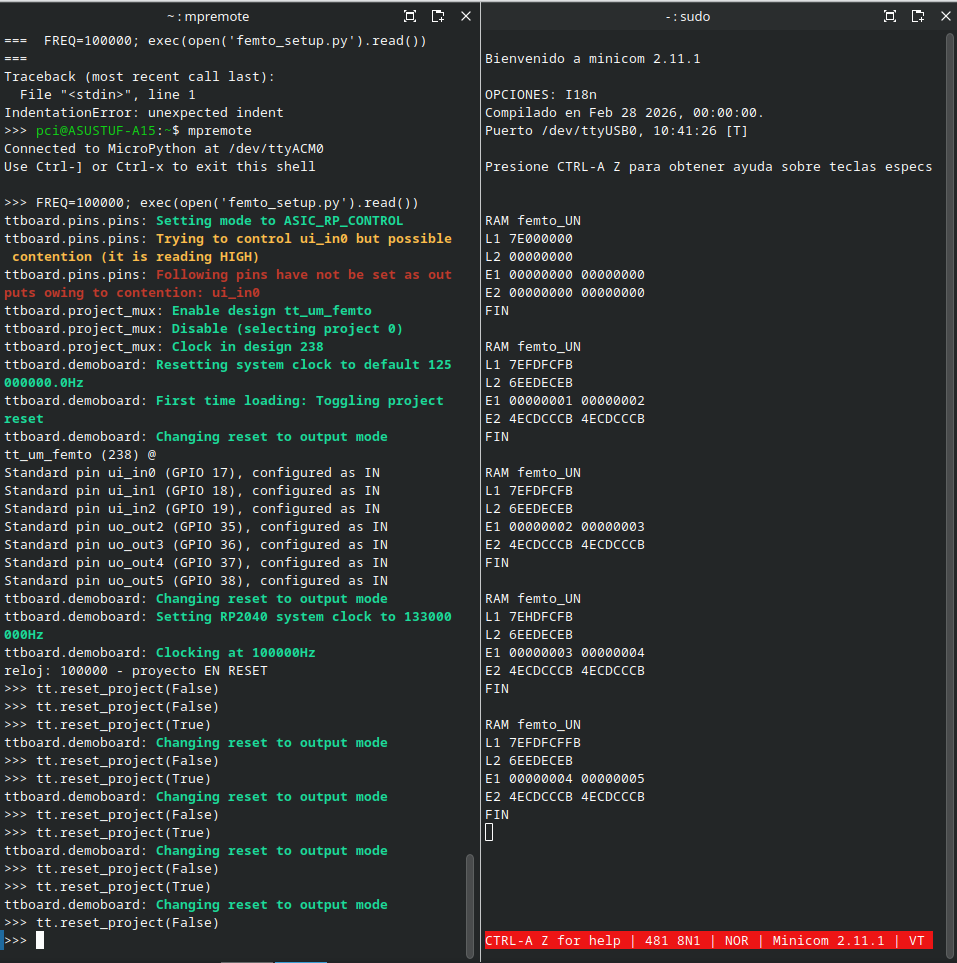
\includegraphics[width=0.62\textwidth]{ram_contador.png}
\caption{Ejecuciones sucesivas de \code{ram\_test.S}: el contador E1 sube en cada reinicio.}
\label{fig:ram_contador}
\end{figure}

\begin{figure}[htbp]
\centering
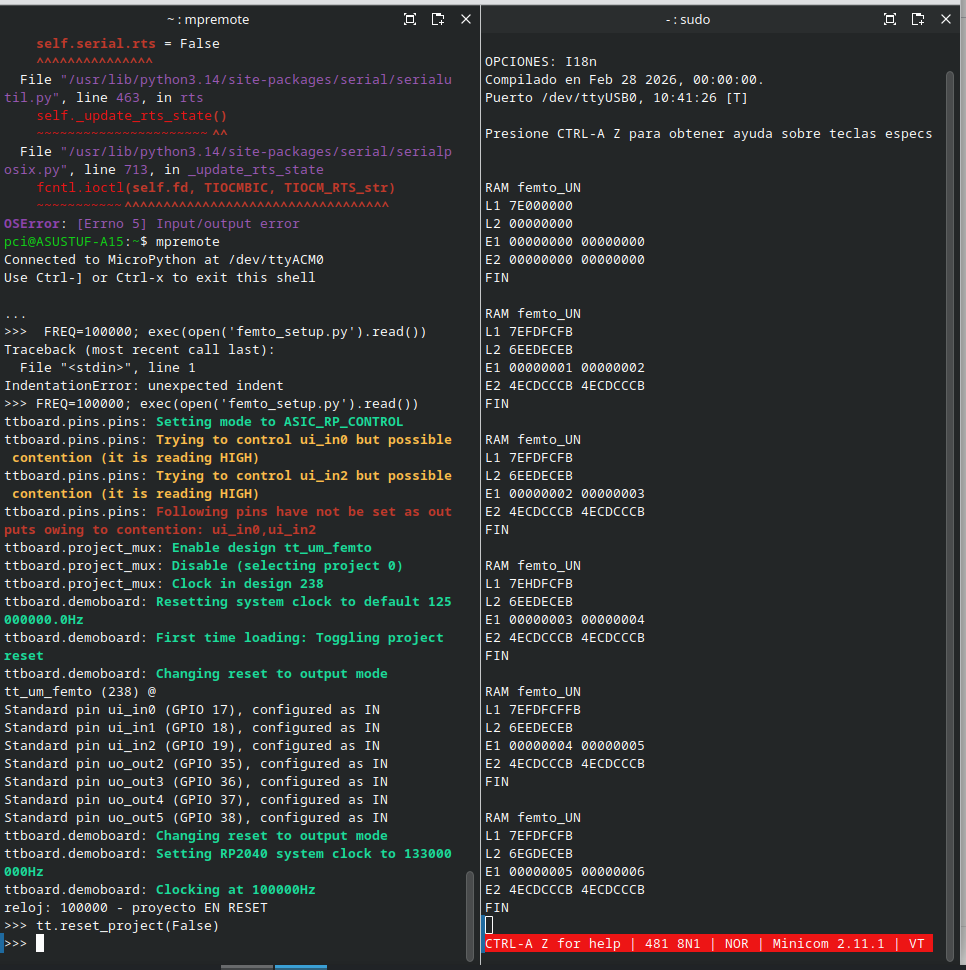
\includegraphics[width=0.62\textwidth]{ram_desconexion.png}
\caption{La misma sesión después de perder la conexión con la placa de demostración: el contador continúa desde el último valor guardado.}
\label{fig:ram_desconexion}
\end{figure}

La primera ejecución muestra solo ceros. En ese momento el cable de 3,3\,V de la RAM no hacía buen contacto; una vez corregido, todas las ejecuciones siguientes funcionaron. A partir de ahí, cada línea confirma una parte de la prueba:

\begin{itemize}
  \item \textbf{Lectura.} L1 y L2 devuelven \code{7EFDFCFB} y \code{6EEDECEB}, los datos que dejó grabados la prueba con el ESP32, con el bit~31 descartado.
  \item \textbf{Escritura.} En E1, el valor releído es siempre el anterior más uno: \code{00000001 00000002}, \code{00000002 00000003}, y así sucesivamente.
  \item \textbf{Necesidad del WREN.} En E2 el valor releído es siempre igual al anterior (\code{4ECDCCCB}). Sin el WREN provocado, la memoria rechaza la escritura.
  \item \textbf{Persistencia.} En la Figura~\ref{fig:ram_desconexion}, la consola de la placa de demostración muestra un error de entrada y salida, porque se perdió la conexión con la placa. Al volver a configurarla y soltar el reset, el contador continúa en \code{00000005 00000006}: el valor escrito se conservó en la memoria ferroeléctrica.
\end{itemize}

En algunas líneas aparecen caracteres alterados, por ejemplo \code{7EHDFCFB}, \code{7EFDFCFFB} o \code{6EGDECEB}. Como el mismo valor se lee correcto en las demás ejecuciones y los caracteres no corresponden a dígitos hexadecimales válidos, se atribuyen a errores de recepción de la UART a 481 baudios y no a la memoria.

\subsection{Transacciones registradas en el analizador}

La captura de PulseView \code{RAM\_1} (10\,s a 1\,MHz) registra el bus de la RAM durante una de esas ejecuciones. El reloj de la RAM mide 9,09\,kHz, y en la captura aparecen las nueve transacciones de la Tabla~\ref{tab:ram1}, una por cada acceso del programa.

\begin{table}[htbp]
\centering
\caption{Transacciones del bus de la RAM en la captura \code{RAM\_1}. Los bytes son los que decodifica PulseView en MOSI y MISO.}
\label{tab:ram1}
{\small
\begin{tabular}{c c l l >{\raggedright\arraybackslash}p{3.6cm}}
\toprule
\textbf{\#} & \textbf{Flancos} & \textbf{MOSI} & \textbf{MISO (últimos bytes)} & \textbf{Interpretación} \\
\midrule
1 & 64 & \code{03 00 00 00 \ldots} & \code{FF FE FD FC FB} & L1: lectura de \code{0x0000} \\
2 & 64 & \code{03 00 10 00 \ldots} & \code{EF EE ED EC EB} & L2: lectura de \code{0x1000} \\
3 & 64 & \code{03 00 20 00 \ldots} & \code{\ldots 00 01} & E1: lectura del contador \\
4 & 63 & \code{06 00 40 00 \ldots} & --- & Lectura en fase mala = WREN \\
5 & 65 & \code{02 00 20 00 00 00 00 02} & --- & E1: escritura del valor 2 \\
6 & 64 & \code{03 00 20 00 \ldots} & \code{\ldots 00 02} & E1: relectura, devuelve 2 \\
7 & 64 & \code{03 00 30 00 \ldots} & \code{CF CE CD CC CB} & E2: lectura del contador \\
8 & 65 & \code{02 00 30 00 4E CD CC CC} & --- & E2: intento de escribir \code{\ldots CC}, sin WREN \\
9 & 64 & \code{03 00 30 00 \ldots} & \code{CF CE CD CC CB} & E2: relectura, sigue en \code{\ldots CB} \\
\bottomrule
\end{tabular}
}
\end{table}

La captura confirma con el propio bus lo que muestra la UART. Las Figuras~\ref{fig:ram_lecturas} a~\ref{fig:ram_e2} muestran esas transacciones en PulseView.

\textbf{Lecturas L1 y L2.} La Figura~\ref{fig:ram_lecturas} muestra las dos lecturas de posiciones fijas. El comando llega completo como \code{03}, seguido de la dirección, y la memoria responde con los datos grabados en la prueba con el ESP32: \code{FF FE FD FC FB} en \code{0x0000} y \code{EF EE ED EC EB} en \code{0x1000}. Una vez descartado el bit~31, son los valores \code{7EFDFCFB} y \code{6EEDECEB} que imprime la UART.

\begin{figure}[htbp]
\centering
\begin{subfigure}[t]{\textwidth}
  \centering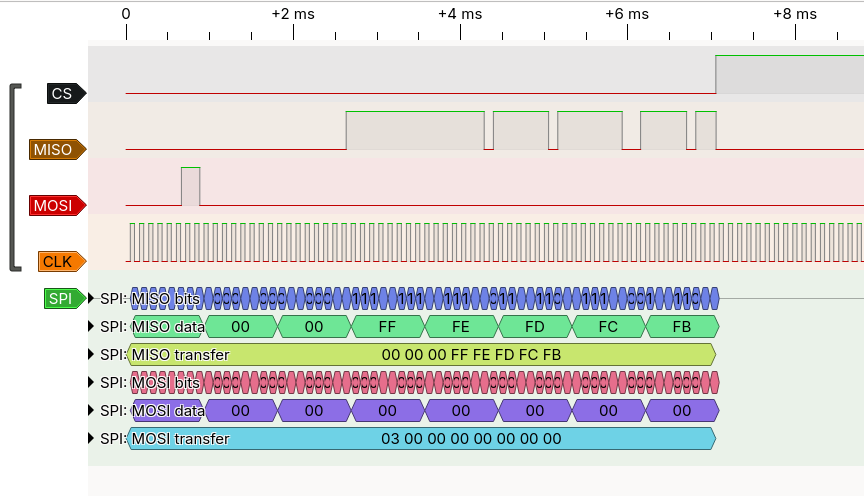
\includegraphics[width=0.78\linewidth]{ram1_l1.png}
  \caption{L1: lectura de \code{0x0000}.}\label{fig:ram_l1}
\end{subfigure}

\vspace{6pt}
\begin{subfigure}[t]{\textwidth}
  \centering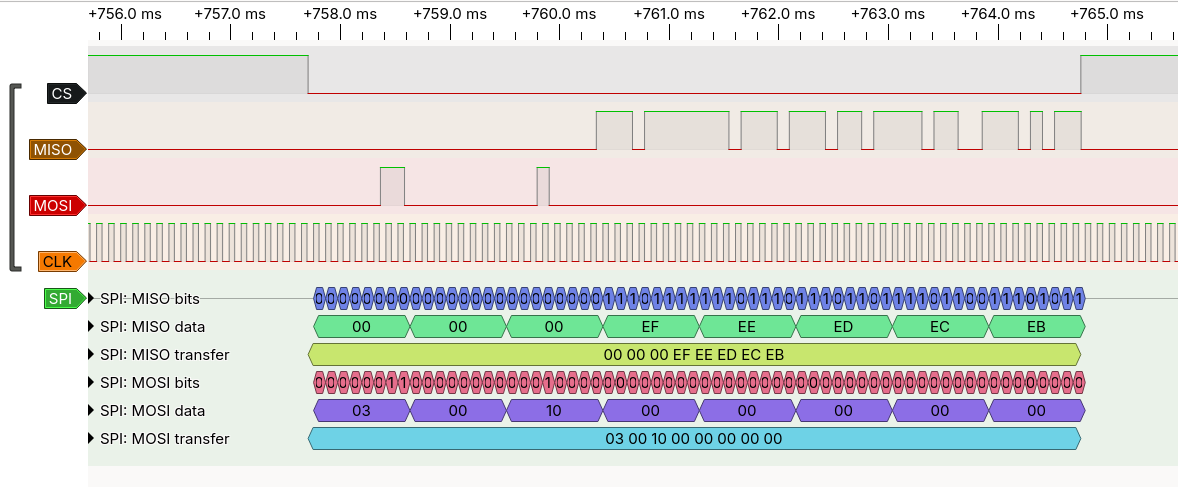
\includegraphics[width=\linewidth]{ram1_l2.png}
  \caption{L2: lectura de \code{0x1000}.}\label{fig:ram_l2}
\end{subfigure}
\caption{Lecturas de posiciones fijas de la RAM en la captura \code{RAM\_1}.}
\label{fig:ram_lecturas}
\end{figure}

\textbf{Contador E1.} La Figura~\ref{fig:ram_e1} muestra el ciclo completo de E1. Primero el programa lee el contador, que vale \code{01}. Luego vienen tres transacciones seguidas. La primera es la lectura en fase mala: tiene 63 flancos en lugar de 64 y PulseView la decodifica como \code{06 00 4\ldots}, que la memoria toma como WREN. La segunda, \code{02 00 2\ldots}, escribe el valor~2. La tercera, \code{03 00 2\ldots}, lo relee, y en MISO aparece el pulso del bit que confirma el nuevo valor.

\begin{figure}[htbp]
\centering
\begin{subfigure}[t]{\textwidth}
  \centering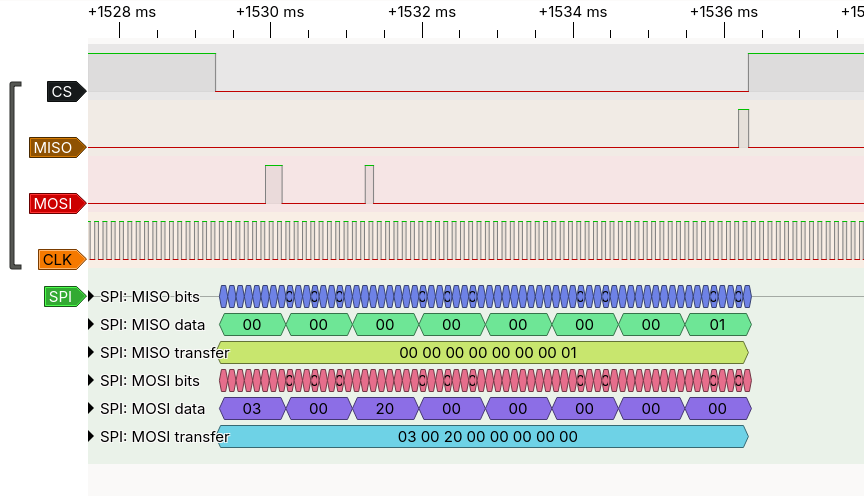
\includegraphics[width=0.78\linewidth]{ram1_e1_lectura.png}
  \caption{Lectura del contador: la memoria devuelve \code{01}.}\label{fig:ram_e1a}
\end{subfigure}

\vspace{6pt}
\begin{subfigure}[t]{\textwidth}
  \centering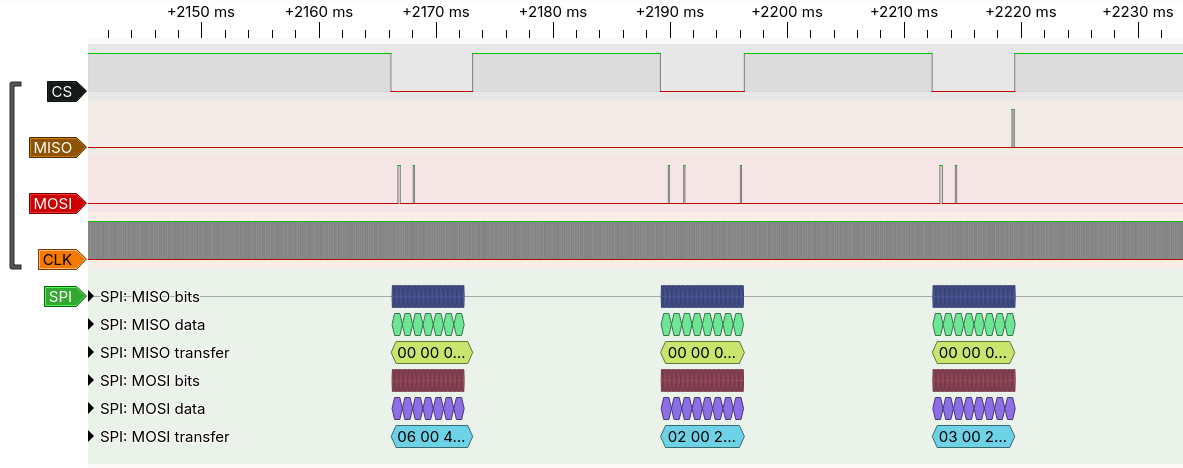
\includegraphics[width=\linewidth]{ram1_e1_secuencia.png}
  \caption{Lectura en fase mala (WREN), escritura del valor~2 y relectura.}\label{fig:ram_e1b}
\end{subfigure}
\caption{Contador E1 con el WREN provocado, en la captura \code{RAM\_1}.}
\label{fig:ram_e1}
\end{figure}

\textbf{Control E2.} La Figura~\ref{fig:ram_e2} muestra la prueba de control. El programa lee el contador (\code{\ldots CF CE CD CC CB}) e intenta escribir \code{4ECDCCCC}, el valor siguiente, sin la lectura en fase mala previa. La relectura devuelve otra vez \code{\ldots CC CB}: sin WREN, la memoria rechazó la escritura.

\begin{figure}[htbp]
\centering
\begin{subfigure}[t]{\textwidth}
  \centering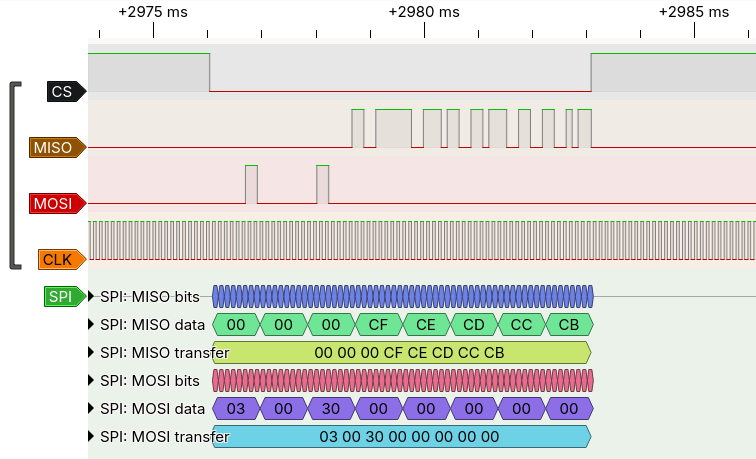
\includegraphics[width=0.7\linewidth]{ram1_e2_lectura.png}
  \caption{Lectura del contador E2.}\label{fig:ram_e2a}
\end{subfigure}

\vspace{6pt}
\begin{subfigure}[t]{\textwidth}
  \centering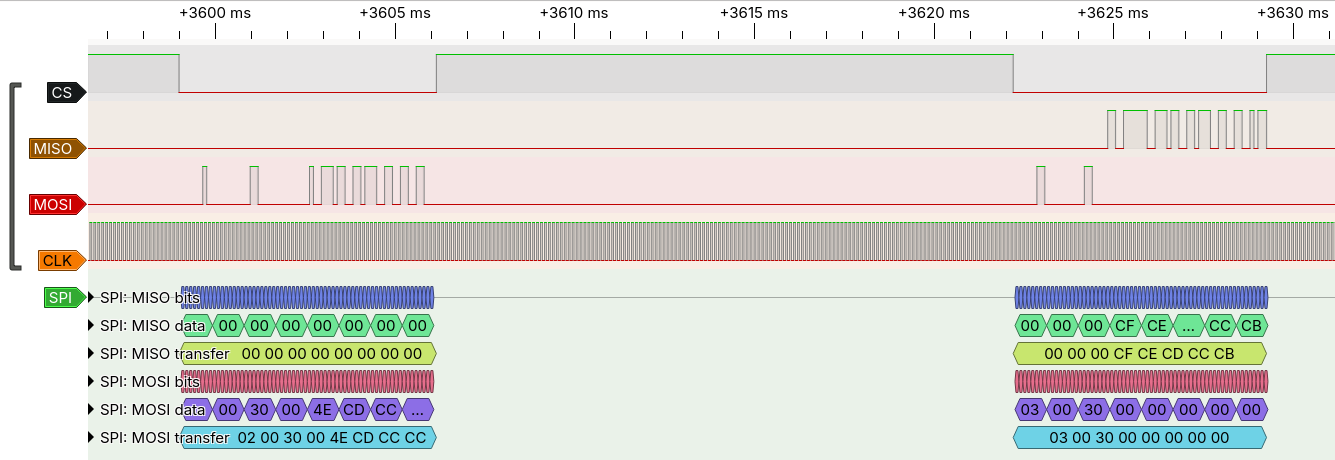
\includegraphics[width=\linewidth]{ram1_e2_escritura.png}
  \caption{Intento de escritura sin WREN y relectura: el valor no cambia.}\label{fig:ram_e2b}
\end{subfigure}
\caption{Prueba de control E2, sin el WREN provocado, en la captura \code{RAM\_1}.}
\label{fig:ram_e2}
\end{figure}

\section{Conversión de texto a mayúsculas}

\subsection{Primera versión}

El segundo programa usa la RAM como almacenamiento de trabajo. Muestra el indicador \code{>}, recibe caracteres por la UART, devuelve el eco de cada uno y lo guarda en la RAM. Al recibir un Enter recorre la memoria, convierte las letras de la \code{a} a la \code{z} en mayúsculas, deja igual los demás caracteres y envía el resultado. Cada escritura va precedida de su WREN provocado, igual que en la prueba anterior.

La primera versión, \code{mayus.S}, funcionó de forma intermitente: con la palabra \code{hola} devolvió \code{HOLA}, pero en otras ejecuciones fallaba sin que se hubiera cambiado nada del montaje.

\subsection{Causa de los fallos}

El origen está en la flash emulada. De vez en cuando el ESP32 no alcanza a atender una lectura de instrucción, y el procesador lee \code{FFFFFFFF}, que ejecuta como un salto hacia atrás (\code{jal x31, -2}). El efecto alterna: unas veces solo reintenta la lectura, y otras ejecuta además la instrucción anterior.

En la prueba anterior eso no tenía consecuencias visibles, pero aquí sí. Una instrucción repetida dura 198 ciclos más, o 201 si es un \code{PAD}, y desplaza la fase del reloj de la RAM. A partir de ese punto todos los \code{PAD} calculados quedan desalineados: el WREN deja de llegar, las escrituras se pierden o las lecturas devuelven datos corridos.

\subsection{Segunda versión}

La versión final, \code{mayus2.S}, está escrita para recuperarse sola de esos fallos en lugar de depender de que no ocurran. Para que repetir una instrucción no haga daño:

\begin{itemize}
  \item Ninguna instrucción escribe un registro que también lee, de modo que ejecutarla dos veces da el mismo resultado.
  \item Antes de cada etiqueta hay un \code{nop}, para que la instrucción que se cuele al saltar hacia atrás sea siempre esa.
  \item No hay subrutinas, porque repetir un \code{jal} repetiría la llamada completa.
  \item No se usa el registro \code{x31}, que es el que escribe el salto provocado por el fallo.
\end{itemize}

Para que una fase desalineada se corrija sola:

\begin{itemize}
  \item \textbf{Escritura comprobada.} Después de cada escritura se relee el dato. Si no coincide, se adelanta la fase un paso con un \code{PAD 1} y se repite, hasta 24 intentos.
  \item \textbf{Dato redundante.} Cada carácter se guarda repetido en cuatro bytes. Al leer se toman dos y se exige que sean iguales y que no sean \code{00} ni \code{FF}, los valores que aparecen cuando la memoria no responde. Si la lectura no pasa la comprobación, también se corre la fase y se repite.
  \item \textbf{Calibración.} Antes de mostrar cada indicador \code{>}, el programa escribe y comprueba una letra de prueba en una posición reservada, para dejar la fase ajustada antes de que llegue el primer carácter.
  \item Si después de 24 intentos un carácter no se puede leer, se envía \code{?} en su lugar.
\end{itemize}

Cada línea admite hasta 50 caracteres; al llegar a ese límite el programa responde sin esperar el Enter.

\subsection{Resultado}

La Figura~\ref{fig:mayus_terminal} muestra una sesión del programa en \code{minicom}. La mayoría de las palabras se devolvieron convertidas a mayúsculas, incluidas frases con espacios como \code{james crack}, \code{eu fallar} y \code{voce falar}. En tres casos la respuesta salió incompleta o vacía: \code{broom} devolvió \code{OM}, y \code{fest} y \code{bruno} no devolvieron texto, aunque al repetir la palabra siguiente (\code{feast}) la conversión volvió a funcionar.

\begin{figure}[htbp]
\centering
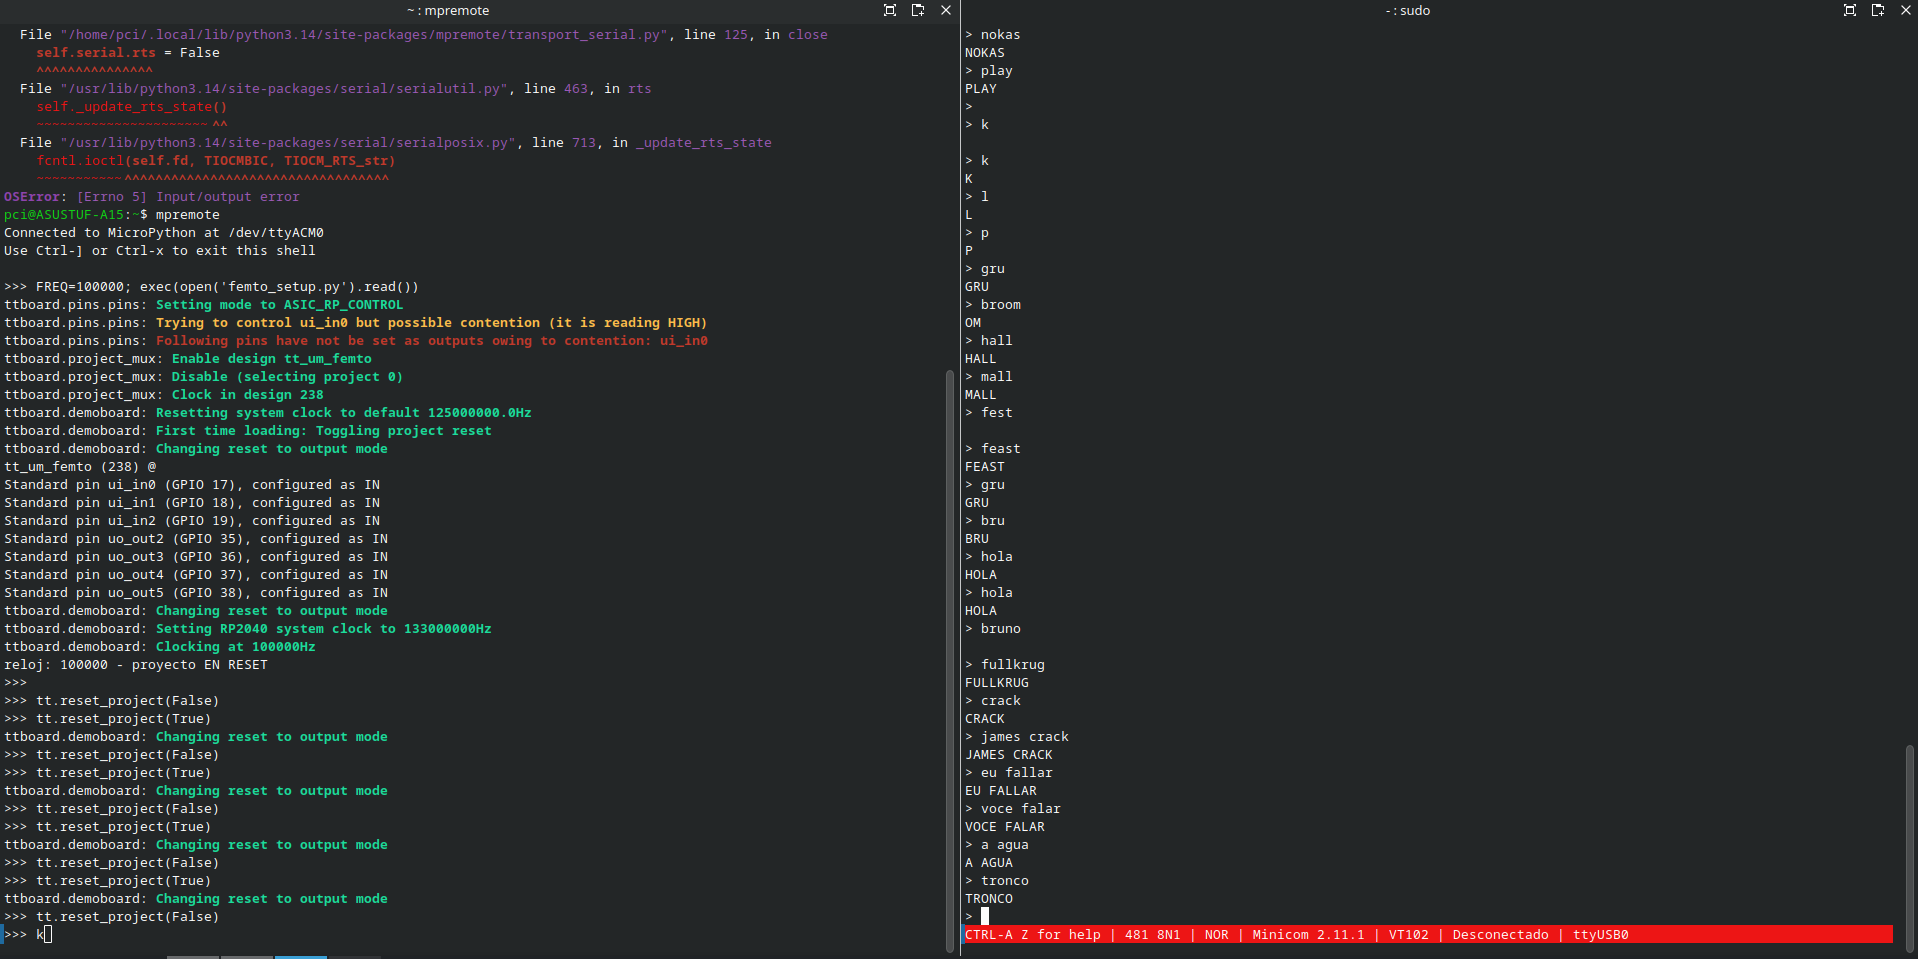
\includegraphics[width=\textwidth]{ram_mayus_terminal.png}
\caption{Sesión del programa de mayúsculas: consola de la placa de demostración (izquierda) y texto enviado y recibido en \code{minicom} (derecha).}
\label{fig:mayus_terminal}
\end{figure}

La captura de PulseView \code{RAM\_HOLA} registra el bus de la RAM mientras se escribe la palabra \code{hola}. La Tabla~\ref{tab:hola} resume sus transacciones. Cada carácter aparece como una lectura en fase mala (WREN), una escritura con el carácter repetido cuatro veces y una relectura que devuelve lo mismo. Al pulsar Enter, el programa vuelve a leer las cuatro posiciones y, antes del siguiente indicador, escribe la letra de calibración \code{Z} (\code{5A}) en la posición reservada \code{0x00FA}. En esta captura todas las escrituras quedaron confirmadas al primer intento.

\begin{table}[htbp]
\centering
\caption{Transacciones del bus de la RAM al escribir \code{hola} (captura \code{RAM\_HOLA}).}
\label{tab:hola}
{\small
\begin{tabular}{r >{\raggedright\arraybackslash}p{4.6cm} l >{\raggedright\arraybackslash}p{4.8cm}}
\toprule
\textbf{Tiempo} & \textbf{Etapa} & \textbf{Dirección} & \textbf{Datos} \\
\midrule
0,02\,s & Escritura de \code{h} y relectura & \code{0x0000} & \code{68 68 68 68} \\
0,62\,s & WREN, escritura de \code{o} y relectura & \code{0x0005} & \code{6F 6F 6F 6F} \\
0,92\,s & WREN, escritura de \code{l} y relectura & \code{0x000A} & \code{6C 6C 6C 6C} \\
1,38\,s & WREN, escritura de \code{a} y relectura & \code{0x000F} & \code{61 61 61 61} \\
2,58--2,92\,s & Enter: lectura de las cuatro posiciones & \code{0x0000}--\code{0x000F} & \code{68}, \code{6F}, \code{6C}, \code{61} \\
3,04\,s & WREN, escritura de calibración y relectura & \code{0x00FA} & \code{5A 5A 5A 5A} (\code{Z}) \\
\bottomrule
\end{tabular}
}
\end{table}

La Figura~\ref{fig:mayus_pv} muestra la vista general de esa actividad en el analizador: cada grupo corresponde a los accesos para guardar o leer un carácter.

\begin{figure}[htbp]
\centering
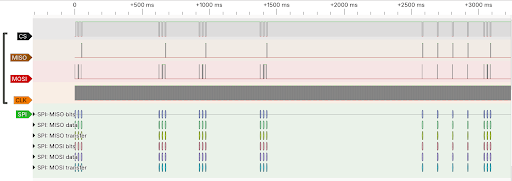
\includegraphics[width=0.9\textwidth]{ram_mayus_pulseview.png}
\caption{Actividad del bus de la RAM durante la conversión a mayúsculas.}
\label{fig:mayus_pv}
\end{figure}

\section{Procedimiento}

\begin{enumerate}
  \item \textbf{Compilar el programa.} Se agrega \code{ram\_test.S} o \code{mayus2.S} al Makefile del firmware en lugar de \code{uart\_full\_demo.S} y se compila con \code{make CROSS=riscv-none-elf}. El proceso genera \code{firmware\_shifted.bin}: 872 bytes para \code{ram\_test.S} y 1004 para \code{mayus2.S}.
  \item \textbf{Cargar el programa en el ESP32-C6.} Se genera \code{firmware.h} con \code{xxd -i} y se carga el mismo emulador del Capítulo~\ref{cap:flash}.
  \item \textbf{Ejecutar.} Igual que en el Capítulo~\ref{cap:flash}: \code{minicom} a 481 baudios en una terminal y, en la consola de la placa de demostración, la configuración seguida de \code{tt.reset\_project(False)}.
  \item Con \code{mayus2.S}, escribir una palabra en \code{minicom} y pulsar Enter.
\end{enumerate}

\section{Problemas encontrados}

{\small
\begin{longtable}{>{\raggedright\arraybackslash}p{4.4cm} >{\raggedright\arraybackslash}p{5cm} >{\raggedright\arraybackslash}p{5cm}}
\caption{Problemas encontrados en la prueba de la RAM.}\label{tab:problemas_ram}\\
\toprule
\textbf{Síntoma} & \textbf{Causa} & \textbf{Solución} \\
\midrule
\endfirsthead
Todas las lecturas y escrituras en cero & El cable de 3,3\,V de la RAM no hacía buen contacto & Corregir la conexión de alimentación \\
Las escrituras no cambian el contenido de la memoria & El controlador del chip no envía WREN & Lectura en fase mala antes de cada escritura \\
La lectura que hace de WREN no cae en fase mala & La fase del reloj de la RAM depende de la secuencia exacta de instrucciones & Ajustar la fase con \code{PAD}, calculado con el modelo ciclo a ciclo \\
Conversión a mayúsculas intermitente & Fallos ocasionales de la flash emulada repiten instrucciones y desalinean la fase & \code{mayus2.S}: código tolerante a repeticiones, escritura comprobada y reintentos \\
Caracteres alterados en la salida de \code{ram\_test.S} & Errores de recepción en la UART a 481 baudios & El valor se confirma en las demás ejecuciones \\
\bottomrule
\end{longtable}
}

% ======================================================================
\chapter{Conclusiones y trabajo futuro}
\label{cap:conclusiones}

\section{Conclusiones}

\begin{itemize}
  \item El femto\_UN fabricado en TTSKY25b funciona en hardware: arranca desde una memoria de programa externa, ejecuta su programa y se comunica por la UART.
  \item El arranque depende de dos condiciones de la memoria de programa: responder solo al comando de lectura y dejar la línea MISO en alto cuando está en reposo. Ambas aplican a cualquier memoria que se conecte al chip, sea el ESP32 o una memoria emulada en una FPGA.
  \item El bus de la RAM funciona: el procesador lee, escribe y conserva datos en la FM25V02. Las capturas del analizador confirman la secuencia WREN, WRITE y READ y que, sin el WREN, la memoria rechaza la escritura.
  \item Escribir depende de un efecto no previsto en el diseño, la pérdida del primer bit del comando. El método funciona, pero obliga a calcular la duración de cada tramo de código y a volver a calcularla con cualquier cambio en los accesos a la RAM.
  \item La versión robusta del programa de mayúsculas paga ese costo en velocidad: cada carácter puede requerir varias escrituras y lecturas antes de quedar confirmado.
  \item Todo se probó a 100\,kHz, limitado por la flash emulada en el ESP32. A la frecuencia de diseño del chip las fases durarían nanosegundos y no se ha comprobado si el método sigue funcionando.
\end{itemize}

\section{Cambios propuestos para una segunda versión}

\begin{itemize}
  \item Detener el reloj SPI entre accesos, en los controladores de flash y de RAM. Con eso desaparecen las fases malas y la necesidad de compensarlas desde el programa.
  \item Enviar el comando WREN antes de cada escritura en el controlador de RAM.
  \item Corregir el muestreo de la línea de datos de la flash, para no tener que grabar el programa corrido un bit.
  \item Permitir las cargas de datos desde la flash, que en este chip no funcionan.
\end{itemize}

% ======================================================================
\begin{thebibliography}{9}
\bibitem{repo_femto} C.~I. Camargo Bareño, \emph{femto\_UN}, repositorio en GitHub. \url{https://github.com/cicamargoba/femto_UN}
\bibitem{repo_shuttle} Tiny Tapeout, \emph{tinytapeout-sky-25b}, repositorio del shuttle TTSKY25b. \url{https://github.com/TinyTapeout/tinytapeout-sky-25b}
\bibitem{tt_chip} Tiny Tapeout, \emph{Tiny Tapeout SKY 25b}, página del shuttle. \url{https://tinytapeout.com/chips/ttsky25b/}
\bibitem{ttsky25b_news} Tiny Tapeout, \emph{TTSKY25b heads to ChipFoundry with 316 designs}, 20 de noviembre de 2025. \url{https://tinytapeout.com/news/ttsky25b-submitted/}
\bibitem{gds_run} GitHub Actions, ejecución del flujo GDS de \code{femto\_UN}. \url{https://github.com/cicamargoba/femto_UN/actions/runs/19103989012}
\end{thebibliography}

\end{document}
